\documentclass[twoside]{book}

% Packages required by doxygen
\usepackage{fixltx2e}
\usepackage{calc}
\usepackage{doxygen}
\usepackage[export]{adjustbox} % also loads graphicx
\usepackage{graphicx}
\usepackage[utf8]{inputenc}
\usepackage{makeidx}
\usepackage{multicol}
\usepackage{multirow}
\PassOptionsToPackage{warn}{textcomp}
\usepackage{textcomp}
\usepackage[nointegrals]{wasysym}
\usepackage[table]{xcolor}

% Font selection
\usepackage[T1]{fontenc}
\usepackage[scaled=.90]{helvet}
\usepackage{courier}
\usepackage{amssymb}
\usepackage{sectsty}
\renewcommand{\familydefault}{\sfdefault}
\allsectionsfont{%
  \fontseries{bc}\selectfont%
  \color{darkgray}%
}
\renewcommand{\DoxyLabelFont}{%
  \fontseries{bc}\selectfont%
  \color{darkgray}%
}
\newcommand{\+}{\discretionary{\mbox{\scriptsize$\hookleftarrow$}}{}{}}

% Page & text layout
\usepackage{geometry}
\geometry{%
  a4paper,%
  top=2.5cm,%
  bottom=2.5cm,%
  left=2.5cm,%
  right=2.5cm%
}
\tolerance=750
\hfuzz=15pt
\hbadness=750
\setlength{\emergencystretch}{15pt}
\setlength{\parindent}{0cm}
\setlength{\parskip}{3ex plus 2ex minus 2ex}
\makeatletter
\renewcommand{\paragraph}{%
  \@startsection{paragraph}{4}{0ex}{-1.0ex}{1.0ex}{%
    \normalfont\normalsize\bfseries\SS@parafont%
  }%
}
\renewcommand{\subparagraph}{%
  \@startsection{subparagraph}{5}{0ex}{-1.0ex}{1.0ex}{%
    \normalfont\normalsize\bfseries\SS@subparafont%
  }%
}
\makeatother

% Headers & footers
\usepackage{fancyhdr}
\pagestyle{fancyplain}
\fancyhead[LE]{\fancyplain{}{\bfseries\thepage}}
\fancyhead[CE]{\fancyplain{}{}}
\fancyhead[RE]{\fancyplain{}{\bfseries\leftmark}}
\fancyhead[LO]{\fancyplain{}{\bfseries\rightmark}}
\fancyhead[CO]{\fancyplain{}{}}
\fancyhead[RO]{\fancyplain{}{\bfseries\thepage}}
\fancyfoot[LE]{\fancyplain{}{}}
\fancyfoot[CE]{\fancyplain{}{}}
\fancyfoot[RE]{\fancyplain{}{\bfseries\scriptsize Generated by Doxygen }}
\fancyfoot[LO]{\fancyplain{}{\bfseries\scriptsize Generated by Doxygen }}
\fancyfoot[CO]{\fancyplain{}{}}
\fancyfoot[RO]{\fancyplain{}{}}
\renewcommand{\footrulewidth}{0.4pt}
\renewcommand{\chaptermark}[1]{%
  \markboth{#1}{}%
}
\renewcommand{\sectionmark}[1]{%
  \markright{\thesection\ #1}%
}

% Indices & bibliography
\usepackage{natbib}
\usepackage[titles]{tocloft}
\setcounter{tocdepth}{3}
\setcounter{secnumdepth}{5}
\makeindex

% Hyperlinks (required, but should be loaded last)
\usepackage{ifpdf}
\ifpdf
  \usepackage[pdftex,pagebackref=true]{hyperref}
\else
  \usepackage[ps2pdf,pagebackref=true]{hyperref}
\fi
\hypersetup{%
  colorlinks=true,%
  linkcolor=blue,%
  citecolor=blue,%
  unicode%
}

% Custom commands
\newcommand{\clearemptydoublepage}{%
  \newpage{\pagestyle{empty}\cleardoublepage}%
}

\usepackage{caption}
\captionsetup{labelsep=space,justification=centering,font={bf},singlelinecheck=off,skip=4pt,position=top}

%===== C O N T E N T S =====

\begin{document}

% Titlepage & ToC
\hypersetup{pageanchor=false,
             bookmarksnumbered=true,
             pdfencoding=unicode
            }
\pagenumbering{alph}
\begin{titlepage}
\vspace*{7cm}
\begin{center}%
{\Large Matrix Library }\\
\vspace*{1cm}
{\large Generated by Doxygen 1.8.13}\\
\end{center}
\end{titlepage}
\clearemptydoublepage
\pagenumbering{roman}
\tableofcontents
\clearemptydoublepage
\pagenumbering{arabic}
\hypersetup{pageanchor=true}

%--- Begin generated contents ---
\chapter{Matrix-\/\+Library}
\label{index}\hypertarget{index}{}A simple Matrix library to perform Matrix Multiplication(using Strassen\textquotesingle{}s Algorithm) and Transpose(Coming Soon !!!). 
\chapter{Namespace Index}
\section{Namespace List}
Here is a list of all namespaces with brief descriptions\+:\begin{DoxyCompactList}
\item\contentsline{section}{\hyperlink{namespaceMATOPS}{M\+A\+T\+O\+PS} \\*The main \hyperlink{matrix_8h}{matrix.\+h} namespace }{\pageref{namespaceMATOPS}}{}
\end{DoxyCompactList}

\chapter{Class Index}
\section{Class List}
Here are the classes, structs, unions and interfaces with brief descriptions\+:\begin{DoxyCompactList}
\item\contentsline{section}{\hyperlink{classMATOPS_1_1BigMatrix}{M\+A\+T\+O\+P\+S\+::\+Big\+Matrix$<$ Data1 $>$} \\*This is the Class for handling Large Matrices. It takes in large Matrices stored as comma-\/separated values (C\+SV) files and perform both Multiplication (Stressan\textquotesingle{}s Algorithm) and transpose }{\pageref{classMATOPS_1_1BigMatrix}}{}
\item\contentsline{section}{\hyperlink{classMATOPS_1_1Matrix}{M\+A\+T\+O\+P\+S\+::\+Matrix$<$ T, m, n $>$} \\*This class is for matrices of smaller size. The user can define a \hyperlink{classMATOPS_1_1Matrix}{Matrix} A of size m x n of Datatype T as follows\+: M\+A\+T\+O\+P\+S\+::\+Matrix$<$\+T,m,n$>$ A }{\pageref{classMATOPS_1_1Matrix}}{}
\end{DoxyCompactList}

\chapter{File Index}
\section{File List}
Here is a list of all documented files with brief descriptions\+:\begin{DoxyCompactList}
\item\contentsline{section}{\hyperlink{example_8cpp}{example.\+cpp} }{\pageref{example_8cpp}}{}
\item\contentsline{section}{\hyperlink{matrix_8h}{matrix.\+h} }{\pageref{matrix_8h}}{}
\end{DoxyCompactList}

\chapter{Namespace Documentation}
\hypertarget{namespaceMATOPS}{}\section{M\+A\+T\+O\+PS Namespace Reference}
\label{namespaceMATOPS}\index{M\+A\+T\+O\+PS@{M\+A\+T\+O\+PS}}


The main \hyperlink{matrix_8h}{matrix.\+h} namespace.  


\subsection*{Classes}
\begin{DoxyCompactItemize}
\item 
class \hyperlink{classMATOPS_1_1BigMatrix}{Big\+Matrix}
\begin{DoxyCompactList}\small\item\em This is the Class for handling Large Matrices. It takes in large Matrices stored as comma-\/separated values (C\+SV) files and perform both Multiplication (Stressan\textquotesingle{}s Algorithm) and transpose. \end{DoxyCompactList}\item 
class \hyperlink{classMATOPS_1_1Matrix}{Matrix}
\begin{DoxyCompactList}\small\item\em This class is for matrices of smaller size. The user can define a \hyperlink{classMATOPS_1_1Matrix}{Matrix} A of size m x n of Datatype T as follows\+: M\+A\+T\+O\+P\+S\+::\+Matrix$<$\+T,m,n$>$ A. \end{DoxyCompactList}\end{DoxyCompactItemize}
\subsection*{Functions}
\begin{DoxyCompactItemize}
\item 
{\footnotesize template$<$typename Data2 $>$ }\\void \hyperlink{namespaceMATOPS_a2050c01cf601a211d3abc45515b8749d}{store\+\_\+csv} (Data2 $\ast$$\ast$C, int m\+\_\+1, int n\+\_\+2, std\+::string path)
\begin{DoxyCompactList}\small\item\em Function template to Store csv file at a given destination file. This function is internally called by matmul and Transpose function (with Data2\+:= int, float etc) to store the Resultant \hyperlink{classMATOPS_1_1BigMatrix}{Big\+Matrix} from the memory to a C\+SV file. \end{DoxyCompactList}\item 
{\footnotesize template$<$typename My\+\_\+data $>$ }\\My\+\_\+data \hyperlink{namespaceMATOPS_a058c07f65db98cd52617d3d5c4de3b42}{convert\+\_\+to} (const std\+::string \&str)
\begin{DoxyCompactList}\small\item\em Function template to convert variable type from string to int,float, double or any other Datatype. \end{DoxyCompactList}\end{DoxyCompactItemize}


\subsection{Detailed Description}
The main \hyperlink{matrix_8h}{matrix.\+h} namespace. 

\subsection{Function Documentation}
\mbox{\Hypertarget{namespaceMATOPS_a058c07f65db98cd52617d3d5c4de3b42}\label{namespaceMATOPS_a058c07f65db98cd52617d3d5c4de3b42}} 
\index{M\+A\+T\+O\+PS@{M\+A\+T\+O\+PS}!convert\+\_\+to@{convert\+\_\+to}}
\index{convert\+\_\+to@{convert\+\_\+to}!M\+A\+T\+O\+PS@{M\+A\+T\+O\+PS}}
\subsubsection{\texorpdfstring{convert\+\_\+to()}{convert\_to()}}
{\footnotesize\ttfamily template$<$typename My\+\_\+data $>$ \\
My\+\_\+data M\+A\+T\+O\+P\+S\+::convert\+\_\+to (\begin{DoxyParamCaption}\item[{const std\+::string \&}]{str }\end{DoxyParamCaption})}



Function template to convert variable type from string to int,float, double or any other Datatype. 


\begin{DoxyTemplParams}{Template Parameters}
{\em My\+\_\+data} & = Datatype into which we want to convert the string input from C\+SV files. \\
\hline
\end{DoxyTemplParams}

\begin{DoxyParams}{Parameters}
{\em str} & = String input from the Csv file. \\
\hline
\end{DoxyParams}
\begin{DoxyReturn}{Returns}
Returns Converted number from string to My\+\_\+data. 
\end{DoxyReturn}

\begin{DoxyCode}
270                         \{
271                                 std::istringstream ss(str);
272 
273                                 My\_data num;
274 
275                                 ss>>num;
276                                 \textcolor{keywordflow}{return} num;
277                         \}
\end{DoxyCode}
\mbox{\Hypertarget{namespaceMATOPS_a2050c01cf601a211d3abc45515b8749d}\label{namespaceMATOPS_a2050c01cf601a211d3abc45515b8749d}} 
\index{M\+A\+T\+O\+PS@{M\+A\+T\+O\+PS}!store\+\_\+csv@{store\+\_\+csv}}
\index{store\+\_\+csv@{store\+\_\+csv}!M\+A\+T\+O\+PS@{M\+A\+T\+O\+PS}}
\subsubsection{\texorpdfstring{store\+\_\+csv()}{store\_csv()}}
{\footnotesize\ttfamily template$<$typename Data2 $>$ \\
void M\+A\+T\+O\+P\+S\+::store\+\_\+csv (\begin{DoxyParamCaption}\item[{Data2 $\ast$$\ast$}]{C,  }\item[{int}]{m\+\_\+1,  }\item[{int}]{n\+\_\+2,  }\item[{std\+::string}]{path }\end{DoxyParamCaption})}



Function template to Store csv file at a given destination file. This function is internally called by matmul and Transpose function (with Data2\+:= int, float etc) to store the Resultant \hyperlink{classMATOPS_1_1BigMatrix}{Big\+Matrix} from the memory to a C\+SV file. 


\begin{DoxyTemplParams}{Template Parameters}
{\em Data2} & \\
\hline
\end{DoxyTemplParams}

\begin{DoxyParams}{Parameters}
{\em C} & = A Pointer pointing to the 2D \hyperlink{classMATOPS_1_1BigMatrix}{Big\+Matrix} in the memory \\
\hline
{\em m\+\_\+1} & = No. of Rows of the Resultant \hyperlink{classMATOPS_1_1BigMatrix}{Big\+Matrix} \\
\hline
{\em n\+\_\+2} & = No. of Columns of the Resultant \hyperlink{classMATOPS_1_1BigMatrix}{Big\+Matrix} \\
\hline
{\em path} & = \char`\"{}path to destination csv file\char`\"{} \\
\hline
\end{DoxyParams}

\begin{DoxyCode}
239                                         \{
240                                                 std::ofstream file;
241                                                 file.open(path);
242 
243                                                 \textcolor{keywordflow}{for}(\textcolor{keywordtype}{int} i=0;i<m\_1;i++)
244                                                 \{
245                                                         \textcolor{keywordflow}{for}(\textcolor{keywordtype}{int} j=0;j<n\_2;j++)
246                                                         \{
247                                                                 file<<C[i][j];
248                                                                 \textcolor{keywordflow}{if}(j<(n\_2)-1)
249                                                                 \{
250                                                                         file<<\textcolor{stringliteral}{","};
251                                                                 \}
252                                                                 \textcolor{keywordflow}{else}
253                                                                 \{
254                                                                         file<<\textcolor{stringliteral}{"\(\backslash\)n"};
255                                                                 \}
256                                                         \}
257                                                 \}
258                                                 file.close();
259 
260                                         \}
\end{DoxyCode}

\chapter{Class Documentation}
\hypertarget{classMATOPS_1_1BigMatrix}{}\section{M\+A\+T\+O\+PS\+:\+:Big\+Matrix$<$ Data1 $>$ Class Template Reference}
\label{classMATOPS_1_1BigMatrix}\index{M\+A\+T\+O\+P\+S\+::\+Big\+Matrix$<$ Data1 $>$@{M\+A\+T\+O\+P\+S\+::\+Big\+Matrix$<$ Data1 $>$}}


This is the Class for handling Large Matrices. It takes in large Matrices stored as comma-\/separated values (C\+SV) files and perform both Multiplication (Stressan\textquotesingle{}s Algorithm) and transpose.  




{\ttfamily \#include $<$matrix.\+h$>$}

\subsection*{Public Member Functions}
\begin{DoxyCompactItemize}
\item 
void \hyperlink{classMATOPS_1_1BigMatrix_a2b3003374e008ff98f763c29aa4e3c07}{Mat\+\_\+print} (std\+::string path)
\begin{DoxyCompactList}\small\item\em Function to print a \hyperlink{classMATOPS_1_1Matrix}{Matrix} from a .csv file. \end{DoxyCompactList}\item 
void \hyperlink{classMATOPS_1_1BigMatrix_a654c6a62d3dec6a4728e56dd361adbf3}{set\+\_\+\+L\+E\+A\+F\+\_\+\+S\+I\+ZE} (int leaf\+\_\+size)
\begin{DoxyCompactList}\small\item\em This Function sets the L\+E\+A\+F\+\_\+\+S\+I\+ZE i.\+e. the array size when we shift from Stressan\textquotesingle{}s Algo to normal O(n$^\wedge$3) solution. The leaf size is used by the Strassen\+Multiply recursive function to manipulate the recursion base condition. Once we reach a square matrix array of size L\+E\+A\+F\+\_\+\+S\+I\+ZE x L\+E\+A\+F\+\_\+\+S\+I\+ZE or lesser, we perform the multiplication using the naive O(n$^\wedge$3) time complexity solution. The value of L\+E\+A\+F\+\_\+\+S\+I\+ZE varies from machine to machine, hence we need to experimentally find out this value for each machine and configure the \hyperlink{matrix_8h}{matrix.\+h} library accordingly. \end{DoxyCompactList}\item 
void \hyperlink{classMATOPS_1_1BigMatrix_a89f5328b2686ef2a0dfaa9c2bd852d37}{set\+\_\+configerd\+\_\+\+Leaf\+\_\+size} ()
\begin{DoxyCompactList}\small\item\em Searches for the configure.\+txt file (generated earlier) and sets the L\+E\+A\+F\+\_\+\+S\+I\+ZE value to the optimal value found out by \hyperlink{configure__lib_8cpp}{configure\+\_\+lib.\+cpp} program during configuration process. This function is called by the \hyperlink{classMATOPS_1_1BigMatrix_ac793236874a8ccfd66e21006011b9cff}{M\+A\+T\+O\+P\+S\+::\+Big\+Matrix$<$\+Data1$>$\+::matmul} before starting the multiplication process. \end{DoxyCompactList}\item 
void \hyperlink{classMATOPS_1_1BigMatrix_ac793236874a8ccfd66e21006011b9cff}{matmul} (std\+::string file\+\_\+1, std\+::string file\+\_\+2, std\+::string path, bool print=false)
\begin{DoxyCompactList}\small\item\em This is the \hyperlink{classMATOPS_1_1BigMatrix}{Big\+Matrix} multiplication Function. To multiply two matrices A and B stored in A.\+csv and B.\+csv respectively and store the result in C.\+csv file. Before brginning the multiplication process it parses the configure.\+txt (generated by \hyperlink{configure__lib_8cpp}{configure\+\_\+lib.\+cpp} during the configuration process) and sets the optimal L\+E\+A\+F\+\_\+\+S\+I\+ZE value. \end{DoxyCompactList}\item 
void \hyperlink{classMATOPS_1_1BigMatrix_a3d3ca40bb701fbc884c6b603dd95e753}{Transpose} (std\+::string path, std\+::string str\+\_\+path)
\begin{DoxyCompactList}\small\item\em This is a function to find the Transpose of a \hyperlink{classMATOPS_1_1BigMatrix}{Big\+Matrix} and stores it in a csv file. \end{DoxyCompactList}\item 
void \hyperlink{classMATOPS_1_1BigMatrix_a1a6d446f0a7e13eae2de1c6702acd706}{Transpose} (std\+::string path)
\begin{DoxyCompactList}\small\item\em This is a function to find the Transpose of a \hyperlink{classMATOPS_1_1BigMatrix}{Big\+Matrix} and stores it in the same csv file (In-\/palce transpose). \end{DoxyCompactList}\end{DoxyCompactItemize}
\subsection*{Private Member Functions}
\begin{DoxyCompactItemize}
\item 
Data1 $\ast$$\ast$ \hyperlink{classMATOPS_1_1BigMatrix_a2730be4ce100cfdbaf1240703bd9cfb9}{Init\+\_\+matrix} (int n)
\begin{DoxyCompactList}\small\item\em Function to dynamically allocate/initialize an n x n matrix in the memory. \end{DoxyCompactList}\item 
Data1 $\ast$$\ast$ \hyperlink{classMATOPS_1_1BigMatrix_a175eecea05e419357d7475f5e3e938da}{add} (Data1 $\ast$$\ast$M1, Data1 $\ast$$\ast$M2, int n)
\begin{DoxyCompactList}\small\item\em Function to Add 2 square Matrices of size n. \end{DoxyCompactList}\item 
Data1 $\ast$$\ast$ \hyperlink{classMATOPS_1_1BigMatrix_a5c89e7f360fb3cc32abbf6f1d430fb1f}{sub} (Data1 $\ast$$\ast$M1, Data1 $\ast$$\ast$M2, int n)
\begin{DoxyCompactList}\small\item\em Function to Subtract 2 square Matrices of size n. \end{DoxyCompactList}\item 
Data1 $\ast$$\ast$ \hyperlink{classMATOPS_1_1BigMatrix_a71c665c80a1ca3731bd0d8ce37f0ace1}{Strassen\+Multiply} (Data1 $\ast$$\ast$A, Data1 $\ast$$\ast$B, int n)
\begin{DoxyCompactList}\small\item\em The main Strassen\textquotesingle{}s Algorithm function implemented using recursion. Takes in square Matrices A and B. \end{DoxyCompactList}\item 
void \hyperlink{classMATOPS_1_1BigMatrix_af5223558c09e6c3c2fd3bcc5ccd08382}{print\+\_\+\+Mat} (Data1 $\ast$$\ast$C, int m, int n)
\begin{DoxyCompactList}\small\item\em This function is called from within the \hyperlink{classMATOPS_1_1BigMatrix_ac793236874a8ccfd66e21006011b9cff}{M\+A\+T\+O\+P\+S\+::\+Big\+Matrix$<$\+Data1$>$\+::matmul} function when print == True. \end{DoxyCompactList}\item 
std\+::vector$<$ std\+::vector$<$ Data1 $>$ $>$ \hyperlink{classMATOPS_1_1BigMatrix_a43e1704cb38eb6d0121be5b71014eb8e}{load\+\_\+\+C\+SV} (const std\+::string \&path)
\begin{DoxyCompactList}\small\item\em Function to load C\+SV file. This function is internally called by \hyperlink{classMATOPS_1_1BigMatrix_ac793236874a8ccfd66e21006011b9cff}{M\+A\+T\+O\+P\+S\+::\+Big\+Matrix$<$\+Data1$>$\+::matmul} and \hyperlink{classMATOPS_1_1BigMatrix_a3d3ca40bb701fbc884c6b603dd95e753}{M\+A\+T\+O\+P\+S\+::\+Big\+Matrix$<$ Data1 $>$\+::\+Transpose} to load the \hyperlink{classMATOPS_1_1BigMatrix}{Big\+Matrix} \textquotesingle{}s to be multiplied or Transposed. It throws an error if path is invalid or C\+SV doesn\textquotesingle{}t exist. \end{DoxyCompactList}\end{DoxyCompactItemize}
\subsection*{Private Attributes}
\begin{DoxyCompactItemize}
\item 
int \hyperlink{classMATOPS_1_1BigMatrix_a3e8820058e3950e17136fd656b97de54}{L\+E\+A\+F\+\_\+\+S\+I\+ZE}
\end{DoxyCompactItemize}


\subsection{Detailed Description}
\subsubsection*{template$<$typename Data1$>$\newline
class M\+A\+T\+O\+P\+S\+::\+Big\+Matrix$<$ Data1 $>$}

This is the Class for handling Large Matrices. It takes in large Matrices stored as comma-\/separated values (C\+SV) files and perform both Multiplication (Stressan\textquotesingle{}s Algorithm) and transpose. 


\begin{DoxyTemplParams}{Template Parameters}
{\em Data1} & = Datatype of the \hyperlink{classMATOPS_1_1BigMatrix}{Big\+Matrix}. Eg. int, float, double etc. \\
\hline
\end{DoxyTemplParams}


\subsection{Member Function Documentation}
\mbox{\Hypertarget{classMATOPS_1_1BigMatrix_a175eecea05e419357d7475f5e3e938da}\label{classMATOPS_1_1BigMatrix_a175eecea05e419357d7475f5e3e938da}} 
\index{M\+A\+T\+O\+P\+S\+::\+Big\+Matrix@{M\+A\+T\+O\+P\+S\+::\+Big\+Matrix}!add@{add}}
\index{add@{add}!M\+A\+T\+O\+P\+S\+::\+Big\+Matrix@{M\+A\+T\+O\+P\+S\+::\+Big\+Matrix}}
\subsubsection{\texorpdfstring{add()}{add()}}
{\footnotesize\ttfamily template$<$typename Data1$>$ \\
Data1$\ast$$\ast$ \hyperlink{classMATOPS_1_1BigMatrix}{M\+A\+T\+O\+P\+S\+::\+Big\+Matrix}$<$ Data1 $>$\+::add (\begin{DoxyParamCaption}\item[{Data1 $\ast$$\ast$}]{M1,  }\item[{Data1 $\ast$$\ast$}]{M2,  }\item[{int}]{n }\end{DoxyParamCaption})\hspace{0.3cm}{\ttfamily [inline]}, {\ttfamily [private]}}



Function to Add 2 square Matrices of size n. 


\begin{DoxyParams}{Parameters}
{\em M1} & = \hyperlink{classMATOPS_1_1BigMatrix}{Big\+Matrix} 1 \\
\hline
{\em M2} & = \hyperlink{classMATOPS_1_1BigMatrix}{Big\+Matrix} 2 \\
\hline
{\em n} & = Size of the Matrices \\
\hline
\end{DoxyParams}
\begin{DoxyReturn}{Returns}
Returns a pointer pointing to the sum of M1 and M2 
\end{DoxyReturn}

\begin{DoxyCode}
323                         \{
324                                 Data1** temp = \hyperlink{classMATOPS_1_1BigMatrix_a2730be4ce100cfdbaf1240703bd9cfb9}{Init\_matrix}(n);
325                             \textcolor{keywordflow}{for}(\textcolor{keywordtype}{int} i=0; i<n; i++)
326                                 \textcolor{keywordflow}{for}(\textcolor{keywordtype}{int} j=0; j<n; j++)
327                                     temp[i][j] = M1[i][j] + M2[i][j];
328                             \textcolor{keywordflow}{return} temp;
329                         \}
\end{DoxyCode}
\mbox{\Hypertarget{classMATOPS_1_1BigMatrix_a2730be4ce100cfdbaf1240703bd9cfb9}\label{classMATOPS_1_1BigMatrix_a2730be4ce100cfdbaf1240703bd9cfb9}} 
\index{M\+A\+T\+O\+P\+S\+::\+Big\+Matrix@{M\+A\+T\+O\+P\+S\+::\+Big\+Matrix}!Init\+\_\+matrix@{Init\+\_\+matrix}}
\index{Init\+\_\+matrix@{Init\+\_\+matrix}!M\+A\+T\+O\+P\+S\+::\+Big\+Matrix@{M\+A\+T\+O\+P\+S\+::\+Big\+Matrix}}
\subsubsection{\texorpdfstring{Init\+\_\+matrix()}{Init\_matrix()}}
{\footnotesize\ttfamily template$<$typename Data1$>$ \\
Data1$\ast$$\ast$ \hyperlink{classMATOPS_1_1BigMatrix}{M\+A\+T\+O\+P\+S\+::\+Big\+Matrix}$<$ Data1 $>$\+::Init\+\_\+matrix (\begin{DoxyParamCaption}\item[{int}]{n }\end{DoxyParamCaption})\hspace{0.3cm}{\ttfamily [inline]}, {\ttfamily [private]}}



Function to dynamically allocate/initialize an n x n matrix in the memory. 


\begin{DoxyParams}{Parameters}
{\em n} & = No. of rows and cols of the \hyperlink{classMATOPS_1_1BigMatrix}{Big\+Matrix}. \\
\hline
\end{DoxyParams}
\begin{DoxyReturn}{Returns}
Returns a pointer pointing to the initialized \hyperlink{classMATOPS_1_1BigMatrix}{Big\+Matrix}. 
\end{DoxyReturn}

\begin{DoxyCode}
303                         \{   \textcolor{comment}{// Calloc chunk of Memory}
304 
305                                 Data1** M;
306                                 M=(Data1 **)calloc(n,\textcolor{keyword}{sizeof}(Data1*)); 
307                                 \textcolor{keywordflow}{for}(\textcolor{keywordtype}{int} i=0;i<n;i++)
308                                 \{
309                                         M[i]=(Data1*)calloc(n,\textcolor{keyword}{sizeof}(Data1));
310                                 \}
311                                 \textcolor{keywordflow}{return} M;
312                         \}
\end{DoxyCode}
\mbox{\Hypertarget{classMATOPS_1_1BigMatrix_a43e1704cb38eb6d0121be5b71014eb8e}\label{classMATOPS_1_1BigMatrix_a43e1704cb38eb6d0121be5b71014eb8e}} 
\index{M\+A\+T\+O\+P\+S\+::\+Big\+Matrix@{M\+A\+T\+O\+P\+S\+::\+Big\+Matrix}!load\+\_\+\+C\+SV@{load\+\_\+\+C\+SV}}
\index{load\+\_\+\+C\+SV@{load\+\_\+\+C\+SV}!M\+A\+T\+O\+P\+S\+::\+Big\+Matrix@{M\+A\+T\+O\+P\+S\+::\+Big\+Matrix}}
\subsubsection{\texorpdfstring{load\+\_\+\+C\+S\+V()}{load\_CSV()}}
{\footnotesize\ttfamily template$<$typename Data1$>$ \\
std\+::vector$<$std\+::vector$<$Data1$>$ $>$ \hyperlink{classMATOPS_1_1BigMatrix}{M\+A\+T\+O\+P\+S\+::\+Big\+Matrix}$<$ Data1 $>$\+::load\+\_\+\+C\+SV (\begin{DoxyParamCaption}\item[{const std\+::string \&}]{path }\end{DoxyParamCaption})\hspace{0.3cm}{\ttfamily [inline]}, {\ttfamily [private]}}



Function to load C\+SV file. This function is internally called by \hyperlink{classMATOPS_1_1BigMatrix_ac793236874a8ccfd66e21006011b9cff}{M\+A\+T\+O\+P\+S\+::\+Big\+Matrix$<$\+Data1$>$\+::matmul} and \hyperlink{classMATOPS_1_1BigMatrix_a3d3ca40bb701fbc884c6b603dd95e753}{M\+A\+T\+O\+P\+S\+::\+Big\+Matrix$<$ Data1 $>$\+::\+Transpose} to load the \hyperlink{classMATOPS_1_1BigMatrix}{Big\+Matrix} \textquotesingle{}s to be multiplied or Transposed. It throws an error if path is invalid or C\+SV doesn\textquotesingle{}t exist. 


\begin{DoxyParams}{Parameters}
{\em path=} & \char`\"{}path to C\+S\+V file i.\+e. to be loaded\char`\"{} \\
\hline
\end{DoxyParams}
\begin{DoxyReturn}{Returns}
A pointer to the \hyperlink{classMATOPS_1_1Matrix}{Matrix} loaded in memory. 
\end{DoxyReturn}

\begin{DoxyCode}
566                 \{
567                     std::ifstream indata;
568                     indata.open(path);
569 
570                     \textcolor{keywordflow}{if}(indata.fail()) \textcolor{comment}{// Check if File exists}
571                     \{
572                         std::cerr<<\textcolor{stringliteral}{"File path: '"}<<path<<\textcolor{stringliteral}{"' doesn't exist\(\backslash\)n"};
573                         exit(0);
574                     \}
575 
576                     std::vector<std::vector<Data1>> dataList;
577                     std::string line = \textcolor{stringliteral}{""};
578 
579                     \textcolor{keywordflow}{while}(getline(indata,line))
580                     \{
581                         std::stringstream lineStream(line);
582                         std::string cell;
583                         std::vector<Data1> temp;
584                         \textcolor{keywordflow}{while} (std::getline(lineStream,cell,\textcolor{charliteral}{','}))
585                         \{
586                             temp.push\_back(convert\_to<Data1>(cell)); \textcolor{comment}{// convert from string to Data1 and
       store it in an 2D array.}
587                         \}
588                         dataList.push\_back(temp);
589 
590                     \}
591                     indata.close(); \textcolor{comment}{// Close file}
592                     \textcolor{keywordflow}{return} dataList; \textcolor{comment}{// Return the 2D vector }
593                 \}
\end{DoxyCode}
\mbox{\Hypertarget{classMATOPS_1_1BigMatrix_a2b3003374e008ff98f763c29aa4e3c07}\label{classMATOPS_1_1BigMatrix_a2b3003374e008ff98f763c29aa4e3c07}} 
\index{M\+A\+T\+O\+P\+S\+::\+Big\+Matrix@{M\+A\+T\+O\+P\+S\+::\+Big\+Matrix}!Mat\+\_\+print@{Mat\+\_\+print}}
\index{Mat\+\_\+print@{Mat\+\_\+print}!M\+A\+T\+O\+P\+S\+::\+Big\+Matrix@{M\+A\+T\+O\+P\+S\+::\+Big\+Matrix}}
\subsubsection{\texorpdfstring{Mat\+\_\+print()}{Mat\_print()}}
{\footnotesize\ttfamily template$<$typename Data1$>$ \\
void \hyperlink{classMATOPS_1_1BigMatrix}{M\+A\+T\+O\+P\+S\+::\+Big\+Matrix}$<$ Data1 $>$\+::Mat\+\_\+print (\begin{DoxyParamCaption}\item[{std\+::string}]{path }\end{DoxyParamCaption})\hspace{0.3cm}{\ttfamily [inline]}}



Function to print a \hyperlink{classMATOPS_1_1Matrix}{Matrix} from a .csv file. 


\begin{DoxyParams}{Parameters}
{\em path} & = \char`\"{}path to .\+csv i.\+e. to be printed\char`\"{} \\
\hline
\end{DoxyParams}

\begin{DoxyCode}
601                 \{
602                         std::vector<std::vector<Data1>> MAT= \hyperlink{classMATOPS_1_1BigMatrix_a43e1704cb38eb6d0121be5b71014eb8e}{load\_CSV}(path);
603 
604                         \textcolor{keywordflow}{for}(std::vector<Data1> a: MAT)
605                         \{
606                                 \textcolor{keywordflow}{for}(Data1 i: a)
607                                 \{
608                                         std::cout<< i <<\textcolor{stringliteral}{" "};
609                                 \}
610                                 std::cout<<\textcolor{charliteral}{'\(\backslash\)n'};
611                         \}
612                 \}
\end{DoxyCode}
\mbox{\Hypertarget{classMATOPS_1_1BigMatrix_ac793236874a8ccfd66e21006011b9cff}\label{classMATOPS_1_1BigMatrix_ac793236874a8ccfd66e21006011b9cff}} 
\index{M\+A\+T\+O\+P\+S\+::\+Big\+Matrix@{M\+A\+T\+O\+P\+S\+::\+Big\+Matrix}!matmul@{matmul}}
\index{matmul@{matmul}!M\+A\+T\+O\+P\+S\+::\+Big\+Matrix@{M\+A\+T\+O\+P\+S\+::\+Big\+Matrix}}
\subsubsection{\texorpdfstring{matmul()}{matmul()}}
{\footnotesize\ttfamily template$<$typename Data1$>$ \\
void \hyperlink{classMATOPS_1_1BigMatrix}{M\+A\+T\+O\+P\+S\+::\+Big\+Matrix}$<$ Data1 $>$\+::matmul (\begin{DoxyParamCaption}\item[{std\+::string}]{file\+\_\+1,  }\item[{std\+::string}]{file\+\_\+2,  }\item[{std\+::string}]{path,  }\item[{bool}]{print = {\ttfamily false} }\end{DoxyParamCaption})\hspace{0.3cm}{\ttfamily [inline]}}



This is the \hyperlink{classMATOPS_1_1BigMatrix}{Big\+Matrix} multiplication Function. To multiply two matrices A and B stored in A.\+csv and B.\+csv respectively and store the result in C.\+csv file. Before brginning the multiplication process it parses the configure.\+txt (generated by \hyperlink{configure__lib_8cpp}{configure\+\_\+lib.\+cpp} during the configuration process) and sets the optimal L\+E\+A\+F\+\_\+\+S\+I\+ZE value. 


\begin{DoxyParams}{Parameters}
{\em file\+\_\+1} & = \char`\"{}path to A.\+csv\char`\"{} \\
\hline
{\em file\+\_\+2} & = \char`\"{}path to B.\+csv\char`\"{} \\
\hline
{\em path} & = path to a store file (no need to predefine C.\+csv file in the directory, it gets generated automatically.) \\
\hline
{\em print} & = True, To see all the Matrices i.\+e. A,B and C in the output terminal/stdio. ~\newline
\begin{DoxyVerb} Define a BigMatrix object BigMatrix<DataType> MatObj, where DataType can be int, float, double, long etc.\n
 Then call MatObj.matmul("path/to/A.csv","path/to/B.csv","path/to/C.csv") from your program. The C.csv file generated file contains C=A*B.\end{DoxyVerb}
 \\
\hline
\end{DoxyParams}

\begin{DoxyCode}
662                                 \{   
663                                         
664 \textcolor{preprocessor}{                                        #ifndef SET\_LEAF\_SIZE }
665                                                 \hyperlink{classMATOPS_1_1BigMatrix_a89f5328b2686ef2a0dfaa9c2bd852d37}{set\_configerd\_Leaf\_size}(); \textcolor{comment}{// Set
       the optimal LEAF\_SIZE by parsing the configuration file genrated by configure\_lib.cpp.}
666 \textcolor{preprocessor}{                                        #endif}
667                                         \textcolor{comment}{// std::cout<<"Current LEAF\_SIZE value: "<<LEAF\_SIZE<<'\(\backslash\)n'; // Just
       a check to see what LEAF\_SIZE value is being used}
668                                         
669                                         \textcolor{comment}{// Parse the CSV files and get the Matrices to be multiplied}
670 
671                                         std::vector<std::vector<Data1>> MAT\_1= 
      \hyperlink{classMATOPS_1_1BigMatrix_a43e1704cb38eb6d0121be5b71014eb8e}{load\_CSV}(file\_1);
672                                         std::vector<std::vector<Data1>> MAT\_2= 
      \hyperlink{classMATOPS_1_1BigMatrix_a43e1704cb38eb6d0121be5b71014eb8e}{load\_CSV}(file\_2);
673 
674                                         \textcolor{comment}{// Get the dimensions of both the Matrices.}
675                                         \textcolor{keywordtype}{int} m\_1=MAT\_1.size(), n\_1=MAT\_1[0].size();  \textcolor{comment}{// Matrix 1 M,N}
676                                         \textcolor{keywordtype}{int} m\_2=MAT\_2.size(), n\_2=MAT\_2[0].size(); \textcolor{comment}{// Matrix 2 M,N}
677 
678                                         \textcolor{keywordflow}{if}(n\_1 != m\_2) \textcolor{comment}{// Check if inner dimensions of the Matrices Match.
       If not then Throw error.}
679                                         \{
680                                                 std::cerr<<\textcolor{stringliteral}{"Matrix Inner Dimensions don't match !!! Matrix
       A dim : "}<<m\_1<<\textcolor{stringliteral}{"x"}<<n\_1<<\textcolor{stringliteral}{" & Matrix B dim : "}<<m\_2<<\textcolor{stringliteral}{"x"}<<n\_2<<\textcolor{stringliteral}{"\(\backslash\)n"};
681                                                 exit(0);
682                                         \}
683                                         \textcolor{keywordflow}{else}  \textcolor{comment}{// Begin Multiplication}
684                                         \{
685                                                 \textcolor{keywordtype}{int} max\_n= std::max(std::max(m\_1,n\_1),n\_2); \textcolor{comment}{// Find the max
       of all the Matrix dimensions, to find the next highest power of 2.}
686                                                 \textcolor{keywordtype}{int} dim\_n=1;
687 
688                                                 \textcolor{comment}{// Find the next highest power of 2 using left shift
       operator (dim\_n = Next highest power of 2).}
689                                                 \textcolor{comment}{// This will be used to pad zeros to both matrices A and B,
       and ultimately given as input to StrassenMultiply() function.}
690                                                 \textcolor{keywordflow}{while}(dim\_n<max\_n)
691                                                 \{
692                                                         dim\_n=dim\_n<<1;
693                                                 \}
694 
695                                                 \textcolor{comment}{// Initialize 3 pointers to point at Matrices A and B, and
       to store the Result of AxB into C.}
696                                                 Data1 ** A;
697                                                 Data1 ** B;
698                                                 Data1 ** C;
699 
700                                                 A=\hyperlink{classMATOPS_1_1BigMatrix_a2730be4ce100cfdbaf1240703bd9cfb9}{Init\_matrix}(dim\_n); \textcolor{comment}{// Allocate the memory for
       Matrix A of size dim\_n}
701                                                 B=\hyperlink{classMATOPS_1_1BigMatrix_a2730be4ce100cfdbaf1240703bd9cfb9}{Init\_matrix}(dim\_n); \textcolor{comment}{// Allocate the memory for
       Matrix B of size dim\_n}
702 
703                                                 \textcolor{comment}{// Build the Zero padded square Matrices A and B}
704                                                         \textcolor{keywordflow}{for}(\textcolor{keywordtype}{int} k=0;k<m\_1;k++)
705                                                         \{
706                                                                 \textcolor{keywordflow}{for}(\textcolor{keywordtype}{int} l=0;l<n\_1;l++)
707                                                                 \{
708                                                                         A[k][l]= MAT\_1[k][l];
709                                                                 \}
710                                                         \}
711 
712                                                         \textcolor{keywordflow}{for}(\textcolor{keywordtype}{int} k=0;k<m\_2;k++)
713                                                         \{
714                                                                 \textcolor{keywordflow}{for}(\textcolor{keywordtype}{int} l=0;l<n\_2;l++)
715                                                                 \{
716                                                                         B[k][l]= MAT\_2[k][l];
717 
718                                                                 \}
719 
720                                                         \}
721 
722                                                 \textcolor{comment}{//Call Stressen's Algorithm function to get A x B and store
       in C.}
723                                                         C=\hyperlink{classMATOPS_1_1BigMatrix_a71c665c80a1ca3731bd0d8ce37f0ace1}{StrassenMultiply}(A, B, dim\_n);
724 
725                                         \textcolor{keywordflow}{if}(print==\textcolor{keyword}{true}) \textcolor{comment}{// if print is true then print A, B and the result
       A.}
726                                                 \{
727                                                                 std::cout<<\textcolor{stringliteral}{"A: \(\backslash\)n"};
728                                                                 \hyperlink{classMATOPS_1_1BigMatrix_af5223558c09e6c3c2fd3bcc5ccd08382}{print\_Mat}(A, m\_1, n\_1); \textcolor{comment}{//Call the
       print\_Mat function to print the Matrix}
729 
730                                                                 std::cout<<\textcolor{stringliteral}{"\(\backslash\)nB: \(\backslash\)n"};
731                                                                 \hyperlink{classMATOPS_1_1BigMatrix_af5223558c09e6c3c2fd3bcc5ccd08382}{print\_Mat}(B, m\_2, n\_2); \textcolor{comment}{//Call the
       print\_Mat function to print the Matrix}
732 
733                                                                 std::cout<<\textcolor{stringliteral}{"\(\backslash\)nANSWER: \(\backslash\)n"}; \textcolor{comment}{//Call the
       print\_Mat function to print the Matrix}
734                                                                 \hyperlink{classMATOPS_1_1BigMatrix_af5223558c09e6c3c2fd3bcc5ccd08382}{print\_Mat}(C, m\_1, n\_2);
735 
736                                                 \}
737 
738                                         \textcolor{comment}{// Store the Result C into a CSV file, whose location is given by
       "path"}
739                                                 store\_csv<Data1>(C, m\_1,n\_2,path);
740 
741                                                 \textcolor{comment}{// Free The memory before quitting}
742                                                 \textcolor{keywordflow}{for}(\textcolor{keywordtype}{int} i=0;i<dim\_n;i++)
743                                                 \{
744                                                         free(A[i]);
745                                                         free(B[i]);
746                                                         free(C[i]);
747                                                 \}
748 
749                                                 free(A);
750                                                 free(B);
751                                                 free(C);
752 
753                                         \}
754 
755                                 \} \textcolor{comment}{// matmul function ends here}
\end{DoxyCode}
\mbox{\Hypertarget{classMATOPS_1_1BigMatrix_af5223558c09e6c3c2fd3bcc5ccd08382}\label{classMATOPS_1_1BigMatrix_af5223558c09e6c3c2fd3bcc5ccd08382}} 
\index{M\+A\+T\+O\+P\+S\+::\+Big\+Matrix@{M\+A\+T\+O\+P\+S\+::\+Big\+Matrix}!print\+\_\+\+Mat@{print\+\_\+\+Mat}}
\index{print\+\_\+\+Mat@{print\+\_\+\+Mat}!M\+A\+T\+O\+P\+S\+::\+Big\+Matrix@{M\+A\+T\+O\+P\+S\+::\+Big\+Matrix}}
\subsubsection{\texorpdfstring{print\+\_\+\+Mat()}{print\_Mat()}}
{\footnotesize\ttfamily template$<$typename Data1$>$ \\
void \hyperlink{classMATOPS_1_1BigMatrix}{M\+A\+T\+O\+P\+S\+::\+Big\+Matrix}$<$ Data1 $>$\+::print\+\_\+\+Mat (\begin{DoxyParamCaption}\item[{Data1 $\ast$$\ast$}]{C,  }\item[{int}]{m,  }\item[{int}]{n }\end{DoxyParamCaption})\hspace{0.3cm}{\ttfamily [inline]}, {\ttfamily [private]}}



This function is called from within the \hyperlink{classMATOPS_1_1BigMatrix_ac793236874a8ccfd66e21006011b9cff}{M\+A\+T\+O\+P\+S\+::\+Big\+Matrix$<$\+Data1$>$\+::matmul} function when print == True. 


\begin{DoxyParams}{Parameters}
{\em C} & \\
\hline
{\em m} & \\
\hline
{\em n} & \\
\hline
\end{DoxyParams}

\begin{DoxyCode}
547                         \{
548                                 \textcolor{keywordflow}{for}(\textcolor{keywordtype}{int} i=0;i<m;i++)
549                                 \{
550                                         \textcolor{keywordflow}{for}(\textcolor{keywordtype}{int} j=0;j<n;j++)
551                                         \{
552                                                 std::cout<<C[i][j]<<\textcolor{stringliteral}{" "};
553                                         \}
554                                         std::cout<<\textcolor{charliteral}{'\(\backslash\)n'};
555                                 \}
556                         \}
\end{DoxyCode}
\mbox{\Hypertarget{classMATOPS_1_1BigMatrix_a89f5328b2686ef2a0dfaa9c2bd852d37}\label{classMATOPS_1_1BigMatrix_a89f5328b2686ef2a0dfaa9c2bd852d37}} 
\index{M\+A\+T\+O\+P\+S\+::\+Big\+Matrix@{M\+A\+T\+O\+P\+S\+::\+Big\+Matrix}!set\+\_\+configerd\+\_\+\+Leaf\+\_\+size@{set\+\_\+configerd\+\_\+\+Leaf\+\_\+size}}
\index{set\+\_\+configerd\+\_\+\+Leaf\+\_\+size@{set\+\_\+configerd\+\_\+\+Leaf\+\_\+size}!M\+A\+T\+O\+P\+S\+::\+Big\+Matrix@{M\+A\+T\+O\+P\+S\+::\+Big\+Matrix}}
\subsubsection{\texorpdfstring{set\+\_\+configerd\+\_\+\+Leaf\+\_\+size()}{set\_configerd\_Leaf\_size()}}
{\footnotesize\ttfamily template$<$typename Data1$>$ \\
void \hyperlink{classMATOPS_1_1BigMatrix}{M\+A\+T\+O\+P\+S\+::\+Big\+Matrix}$<$ Data1 $>$\+::set\+\_\+configerd\+\_\+\+Leaf\+\_\+size (\begin{DoxyParamCaption}{ }\end{DoxyParamCaption})\hspace{0.3cm}{\ttfamily [inline]}}



Searches for the configure.\+txt file (generated earlier) and sets the L\+E\+A\+F\+\_\+\+S\+I\+ZE value to the optimal value found out by \hyperlink{configure__lib_8cpp}{configure\+\_\+lib.\+cpp} program during configuration process. This function is called by the \hyperlink{classMATOPS_1_1BigMatrix_ac793236874a8ccfd66e21006011b9cff}{M\+A\+T\+O\+P\+S\+::\+Big\+Matrix$<$\+Data1$>$\+::matmul} before starting the multiplication process. 


\begin{DoxyCode}
637                 \{
638                         std::ifstream indata;
639                         indata.open(\textcolor{stringliteral}{"configure.txt"});
640                         std::string str=\textcolor{stringliteral}{""};
641                         getline(indata,str);
642                         indata.close();
643                         \hyperlink{classMATOPS_1_1BigMatrix_a3e8820058e3950e17136fd656b97de54}{LEAF\_SIZE}=std::stoi(str);
644                 \}
\end{DoxyCode}
\mbox{\Hypertarget{classMATOPS_1_1BigMatrix_a654c6a62d3dec6a4728e56dd361adbf3}\label{classMATOPS_1_1BigMatrix_a654c6a62d3dec6a4728e56dd361adbf3}} 
\index{M\+A\+T\+O\+P\+S\+::\+Big\+Matrix@{M\+A\+T\+O\+P\+S\+::\+Big\+Matrix}!set\+\_\+\+L\+E\+A\+F\+\_\+\+S\+I\+ZE@{set\+\_\+\+L\+E\+A\+F\+\_\+\+S\+I\+ZE}}
\index{set\+\_\+\+L\+E\+A\+F\+\_\+\+S\+I\+ZE@{set\+\_\+\+L\+E\+A\+F\+\_\+\+S\+I\+ZE}!M\+A\+T\+O\+P\+S\+::\+Big\+Matrix@{M\+A\+T\+O\+P\+S\+::\+Big\+Matrix}}
\subsubsection{\texorpdfstring{set\+\_\+\+L\+E\+A\+F\+\_\+\+S\+I\+Z\+E()}{set\_LEAF\_SIZE()}}
{\footnotesize\ttfamily template$<$typename Data1$>$ \\
void \hyperlink{classMATOPS_1_1BigMatrix}{M\+A\+T\+O\+P\+S\+::\+Big\+Matrix}$<$ Data1 $>$\+::set\+\_\+\+L\+E\+A\+F\+\_\+\+S\+I\+ZE (\begin{DoxyParamCaption}\item[{int}]{leaf\+\_\+size }\end{DoxyParamCaption})\hspace{0.3cm}{\ttfamily [inline]}}



This Function sets the L\+E\+A\+F\+\_\+\+S\+I\+ZE i.\+e. the array size when we shift from Stressan\textquotesingle{}s Algo to normal O(n$^\wedge$3) solution. The leaf size is used by the Strassen\+Multiply recursive function to manipulate the recursion base condition. Once we reach a square matrix array of size L\+E\+A\+F\+\_\+\+S\+I\+ZE x L\+E\+A\+F\+\_\+\+S\+I\+ZE or lesser, we perform the multiplication using the naive O(n$^\wedge$3) time complexity solution. The value of L\+E\+A\+F\+\_\+\+S\+I\+ZE varies from machine to machine, hence we need to experimentally find out this value for each machine and configure the \hyperlink{matrix_8h}{matrix.\+h} library accordingly. 

The S\+E\+T\+\_\+\+L\+E\+A\+F\+\_\+\+S\+I\+ZE flag is raised by \hyperlink{configure__lib_8cpp}{configure\+\_\+lib.\+cpp} file during execution, thus allowing it to manipulate the L\+E\+A\+F\+\_\+\+S\+I\+ZE (private variable) of the \hyperlink{matrix_8h}{matrix.\+h} file . Hence configure.\+cpp can test the hardware for different values of L\+E\+A\+F\+\_\+\+S\+I\+ZE and pick the optimal L\+E\+A\+F\+\_\+\+S\+I\+ZE value (i.\+e. the one with the lowest execution time) and generate the configure.\+txt file. 
\begin{DoxyCode}
627                 \{
628                         \hyperlink{classMATOPS_1_1BigMatrix_a3e8820058e3950e17136fd656b97de54}{LEAF\_SIZE}=leaf\_size;
629                 \}
\end{DoxyCode}
\mbox{\Hypertarget{classMATOPS_1_1BigMatrix_a71c665c80a1ca3731bd0d8ce37f0ace1}\label{classMATOPS_1_1BigMatrix_a71c665c80a1ca3731bd0d8ce37f0ace1}} 
\index{M\+A\+T\+O\+P\+S\+::\+Big\+Matrix@{M\+A\+T\+O\+P\+S\+::\+Big\+Matrix}!Strassen\+Multiply@{Strassen\+Multiply}}
\index{Strassen\+Multiply@{Strassen\+Multiply}!M\+A\+T\+O\+P\+S\+::\+Big\+Matrix@{M\+A\+T\+O\+P\+S\+::\+Big\+Matrix}}
\subsubsection{\texorpdfstring{Strassen\+Multiply()}{StrassenMultiply()}}
{\footnotesize\ttfamily template$<$typename Data1$>$ \\
Data1$\ast$$\ast$ \hyperlink{classMATOPS_1_1BigMatrix}{M\+A\+T\+O\+P\+S\+::\+Big\+Matrix}$<$ Data1 $>$\+::Strassen\+Multiply (\begin{DoxyParamCaption}\item[{Data1 $\ast$$\ast$}]{A,  }\item[{Data1 $\ast$$\ast$}]{B,  }\item[{int}]{n }\end{DoxyParamCaption})\hspace{0.3cm}{\ttfamily [inline]}, {\ttfamily [private]}}



The main Strassen\textquotesingle{}s Algorithm function implemented using recursion. Takes in square Matrices A and B. 


\begin{DoxyParams}{Parameters}
{\em A} & = \hyperlink{classMATOPS_1_1BigMatrix}{Big\+Matrix} A \\
\hline
{\em B} & = \hyperlink{classMATOPS_1_1BigMatrix}{Big\+Matrix} B \\
\hline
{\em n} & = Size of both A and B \\
\hline
\end{DoxyParams}
\begin{DoxyReturn}{Returns}
Returns a square matrix i.\+e. the Multiplication result of A and B. 
\end{DoxyReturn}

\begin{DoxyCode}
356                         \{   
357                                 \textcolor{comment}{/* Naive Stressan's Algorithm (more time consuming)}
358 \textcolor{comment}{                                  if(n==1)}
359 \textcolor{comment}{                                \{}
360 \textcolor{comment}{                                        Data1** C=Init\_matrix(1);}
361 \textcolor{comment}{                                        C[0][0]=A[0][0]*B[0][0];}
362 \textcolor{comment}{                                        return C;}
363 \textcolor{comment}{                                \}*/}
364 
365                                 \textcolor{comment}{// Once array size of LEAF\_SIZE x LEAF\_SIZE or lesser is reached we switch
       to the O(n^3) Matrix Multiplication solution, since after this }
366                                 \textcolor{comment}{// stage the recursion calls become a burden to the whole algorithm and we
       end up getting high execution time. This value of "64" is }
367                                 \textcolor{comment}{// architecture dependent and will vary from machine to machine.}
368                                 \textcolor{keywordflow}{if}(n<=\hyperlink{classMATOPS_1_1BigMatrix_a3e8820058e3950e17136fd656b97de54}{LEAF\_SIZE})
369                                 \{
370                                         Data1** C=\hyperlink{classMATOPS_1_1BigMatrix_a2730be4ce100cfdbaf1240703bd9cfb9}{Init\_matrix}(n);
371                                         \textcolor{keywordflow}{for}(\textcolor{keywordtype}{int} i=0;i<n;i++)
372                                         \{
373                                                 \textcolor{keywordflow}{for}(\textcolor{keywordtype}{int} j=0;j<n;j++)
374                                                 \{
375                                                         \textcolor{keywordflow}{for}(\textcolor{keywordtype}{int} k=0;k<n;k++)
376                                                         \{
377                                                                 C[i][j]+=A[i][k]*B[k][j];
378                                                         \}
379                                                 \}
380                                         \}
381                                         \textcolor{keywordflow}{return} C;
382                                 \}
383 
384                                 Data1** C = \hyperlink{classMATOPS_1_1BigMatrix_a2730be4ce100cfdbaf1240703bd9cfb9}{Init\_matrix}(n); \textcolor{comment}{// Initialize an nxn matrix to store
       }
385                                 \textcolor{keywordtype}{int} k = n/2;
386 
387                                 \textcolor{comment}{// Initialize the Block Matrices}
388                                 Data1** A11 = \hyperlink{classMATOPS_1_1BigMatrix_a2730be4ce100cfdbaf1240703bd9cfb9}{Init\_matrix}(k);
389                                 Data1** A12 = \hyperlink{classMATOPS_1_1BigMatrix_a2730be4ce100cfdbaf1240703bd9cfb9}{Init\_matrix}(k);
390                                 Data1** A21 = \hyperlink{classMATOPS_1_1BigMatrix_a2730be4ce100cfdbaf1240703bd9cfb9}{Init\_matrix}(k);
391                                 Data1** A22 = \hyperlink{classMATOPS_1_1BigMatrix_a2730be4ce100cfdbaf1240703bd9cfb9}{Init\_matrix}(k);
392                                 Data1** B11 = \hyperlink{classMATOPS_1_1BigMatrix_a2730be4ce100cfdbaf1240703bd9cfb9}{Init\_matrix}(k);
393                                 Data1** B12 = \hyperlink{classMATOPS_1_1BigMatrix_a2730be4ce100cfdbaf1240703bd9cfb9}{Init\_matrix}(k);
394                                 Data1** B21 = \hyperlink{classMATOPS_1_1BigMatrix_a2730be4ce100cfdbaf1240703bd9cfb9}{Init\_matrix}(k);
395                                 Data1** B22 = \hyperlink{classMATOPS_1_1BigMatrix_a2730be4ce100cfdbaf1240703bd9cfb9}{Init\_matrix}(k);
396 
397                                 \textcolor{comment}{// Build the block Matrices}
398                                 \textcolor{keywordflow}{for}(\textcolor{keywordtype}{int} i=0;i<k;i++)
399                                 \{
400                                         \textcolor{keywordflow}{for}(\textcolor{keywordtype}{int} j=0;j<k;j++)
401                                         \{
402                                                 A11[i][j] = A[i][j];
403                                                 A12[i][j] = A[i][k+j];
404                                                 A21[i][j] = A[k+i][j];
405                                                 A22[i][j] = A[k+i][k+j];
406                                                 B11[i][j] = B[i][j];
407                                                 B12[i][j] = B[i][k+j];
408                                                 B21[i][j] = B[k+i][j];
409                                                 B22[i][j] = B[k+i][k+j];
410                                         \}
411                                 \}
412                                 \textcolor{comment}{// Determine the Strassen's Coefficients}
413                                 Data1** TEMP\_B12\_B22 = \hyperlink{classMATOPS_1_1BigMatrix_a5c89e7f360fb3cc32abbf6f1d430fb1f}{sub}(B12, B22, k);
414                                 Data1** TEMP\_A11\_A12 = \hyperlink{classMATOPS_1_1BigMatrix_a175eecea05e419357d7475f5e3e938da}{add}(A11, A12, k);
415                                 Data1** TEMP\_A21\_A22 = \hyperlink{classMATOPS_1_1BigMatrix_a175eecea05e419357d7475f5e3e938da}{add}(A21, A22, k);
416                                 Data1** TEMP\_B21\_B11 = \hyperlink{classMATOPS_1_1BigMatrix_a5c89e7f360fb3cc32abbf6f1d430fb1f}{sub}(B21, B11, k);
417 
418 
419                                 Data1** P1 = \hyperlink{classMATOPS_1_1BigMatrix_a71c665c80a1ca3731bd0d8ce37f0ace1}{StrassenMultiply}(A11, TEMP\_B12\_B22, k);
420                                 Data1** P2 = \hyperlink{classMATOPS_1_1BigMatrix_a71c665c80a1ca3731bd0d8ce37f0ace1}{StrassenMultiply}(TEMP\_A11\_A12, B22, k);
421                                 Data1** P3 = \hyperlink{classMATOPS_1_1BigMatrix_a71c665c80a1ca3731bd0d8ce37f0ace1}{StrassenMultiply}(TEMP\_A21\_A22, B11, k);
422                                 Data1** P4 = \hyperlink{classMATOPS_1_1BigMatrix_a71c665c80a1ca3731bd0d8ce37f0ace1}{StrassenMultiply}(A22, TEMP\_B21\_B11, k);
423 
424                                 Data1** TEMP\_A11\_A22 = \hyperlink{classMATOPS_1_1BigMatrix_a175eecea05e419357d7475f5e3e938da}{add}(A11, A22, k);
425                                 Data1** TEMP\_B11\_B22 = \hyperlink{classMATOPS_1_1BigMatrix_a175eecea05e419357d7475f5e3e938da}{add}(B11, B22, k);
426                                 Data1** TEMP\_A12\_A22 = \hyperlink{classMATOPS_1_1BigMatrix_a5c89e7f360fb3cc32abbf6f1d430fb1f}{sub}(A12, A22, k);
427                                 Data1** TEMP\_B21\_B22 = \hyperlink{classMATOPS_1_1BigMatrix_a175eecea05e419357d7475f5e3e938da}{add}(B21, B22, k);
428                                 Data1** TEMP\_A11\_A21 = \hyperlink{classMATOPS_1_1BigMatrix_a5c89e7f360fb3cc32abbf6f1d430fb1f}{sub}(A11, A21, k);
429                                 Data1** TEMP\_B11\_B12 = \hyperlink{classMATOPS_1_1BigMatrix_a175eecea05e419357d7475f5e3e938da}{add}(B11, B12, k);
430 
431                                 Data1** P5 = \hyperlink{classMATOPS_1_1BigMatrix_a71c665c80a1ca3731bd0d8ce37f0ace1}{StrassenMultiply}(TEMP\_A11\_A22, TEMP\_B11\_B22, k
      );
432                                 Data1** P6 = \hyperlink{classMATOPS_1_1BigMatrix_a71c665c80a1ca3731bd0d8ce37f0ace1}{StrassenMultiply}(TEMP\_A12\_A22, TEMP\_B21\_B22, k
      );
433                                 Data1** P7 = \hyperlink{classMATOPS_1_1BigMatrix_a71c665c80a1ca3731bd0d8ce37f0ace1}{StrassenMultiply}(TEMP\_A11\_A21, TEMP\_B11\_B12, k
      );
434 
435                                 Data1** TEMP\_P5\_P4 = \hyperlink{classMATOPS_1_1BigMatrix_a175eecea05e419357d7475f5e3e938da}{add}(P5, P4, k);
436                                 Data1** TEMP\_P5\_P4\_P6 = \hyperlink{classMATOPS_1_1BigMatrix_a175eecea05e419357d7475f5e3e938da}{add}(TEMP\_P5\_P4, P6, k);
437                                 Data1** TEMP\_P5\_P1 = \hyperlink{classMATOPS_1_1BigMatrix_a175eecea05e419357d7475f5e3e938da}{add}(P5, P1, k);
438                                 Data1** TEMP\_P5\_P1\_P3 = \hyperlink{classMATOPS_1_1BigMatrix_a5c89e7f360fb3cc32abbf6f1d430fb1f}{sub}(TEMP\_P5\_P1, P3, k);
439 
440 
441                                 Data1** C11 = \hyperlink{classMATOPS_1_1BigMatrix_a5c89e7f360fb3cc32abbf6f1d430fb1f}{sub}(TEMP\_P5\_P4\_P6, P2, k);
442                                 Data1** C12 = \hyperlink{classMATOPS_1_1BigMatrix_a175eecea05e419357d7475f5e3e938da}{add}(P1, P2, k);
443                                 Data1** C21 = \hyperlink{classMATOPS_1_1BigMatrix_a175eecea05e419357d7475f5e3e938da}{add}(P3, P4, k);
444                                 Data1** C22 = \hyperlink{classMATOPS_1_1BigMatrix_a5c89e7f360fb3cc32abbf6f1d430fb1f}{sub}(TEMP\_P5\_P1\_P3, P7, k);
445 
446                                 \textcolor{comment}{// Building the returning C Matrix}
447 
448                                 \textcolor{keywordflow}{for}(\textcolor{keywordtype}{int} i=0; i<k; i++)
449                                 \{
450                                         \textcolor{keywordflow}{for}(\textcolor{keywordtype}{int} j=0; j<k; j++)
451                                         \{
452                                                 C[i][j] = C11[i][j];
453                                                 C[i][j+k] = C12[i][j];
454                                                 C[k+i][j] = C21[i][j];
455                                                 C[k+i][k+j] = C22[i][j];
456                                         \}
457                                 \}
458 
459                                 \textcolor{comment}{// Free up all calloced memory.}
460                                 \textcolor{keywordflow}{for}(\textcolor{keywordtype}{int} i=0; i<k; i++) \{
461                                                 free(TEMP\_B12\_B22[i]);
462                                                 free(TEMP\_A11\_A12[i]);
463                                                 free(TEMP\_A21\_A22[i]);
464                                                 free(TEMP\_B21\_B11[i]);
465 
466                                                 free(TEMP\_A11\_A22[i]);
467                                                 free(TEMP\_B11\_B22[i]);
468                                                 free(TEMP\_A12\_A22[i]);
469                                                 free(TEMP\_B21\_B22[i]);
470                                                 free(TEMP\_A11\_A21[i]);
471                                                 free(TEMP\_B11\_B12[i]);
472 
473                                                 free(TEMP\_P5\_P4[i]);
474                                                 free(TEMP\_P5\_P4\_P6[i]);
475                                                 free(TEMP\_P5\_P1[i]);
476                                                 free(TEMP\_P5\_P1\_P3[i]);
477 
478                                         free(A11[i]);
479                                         free(A12[i]);
480                                         free(A21[i]);
481                                         free(A22[i]);
482                                         free(B11[i]);
483                                         free(B12[i]);
484                                         free(B21[i]);
485                                         free(B22[i]);
486                                         free(P1[i]);
487                                         free(P2[i]);
488                                         free(P3[i]);
489                                         free(P4[i]);
490                                         free(P5[i]);
491                                         free(P6[i]);
492                                         free(P7[i]);
493                                         free(C11[i]);
494                                         free(C12[i]);
495                                         free(C21[i]);
496                                         free(C22[i]);
497                                     \}
498 
499                                         free(TEMP\_B12\_B22);
500                                         free(TEMP\_A11\_A12);
501                                         free(TEMP\_A21\_A22);
502                                         free(TEMP\_B21\_B11);
503 
504                                         free(TEMP\_A11\_A22);
505                                         free(TEMP\_B11\_B22);
506                                         free(TEMP\_A12\_A22);
507                                         free(TEMP\_B21\_B22);
508                                         free(TEMP\_A11\_A21);
509                                         free(TEMP\_B11\_B12);
510 
511                                         free(TEMP\_P5\_P4);
512                                         free(TEMP\_P5\_P4\_P6);
513                                         free(TEMP\_P5\_P1);
514                                         free(TEMP\_P5\_P1\_P3);
515 
516                                         free(A11);
517                                     free(A12);
518                                     free(A21);
519                                     free(A22);
520                                     free(B11);
521                                     free(B12);
522                                     free(B21);
523                                     free(B22);
524                                     free(P1);
525                                     free(P2);
526                                     free(P3);
527                                     free(P4);
528                                     free(P5);
529                                     free(P6);
530                                     free(P7);
531                                     free(C11);
532                                     free(C12);
533                                     free(C21);
534                                     free(C22);
535 
536                                     \textcolor{keywordflow}{return} C;
537                         \}
\end{DoxyCode}
\mbox{\Hypertarget{classMATOPS_1_1BigMatrix_a5c89e7f360fb3cc32abbf6f1d430fb1f}\label{classMATOPS_1_1BigMatrix_a5c89e7f360fb3cc32abbf6f1d430fb1f}} 
\index{M\+A\+T\+O\+P\+S\+::\+Big\+Matrix@{M\+A\+T\+O\+P\+S\+::\+Big\+Matrix}!sub@{sub}}
\index{sub@{sub}!M\+A\+T\+O\+P\+S\+::\+Big\+Matrix@{M\+A\+T\+O\+P\+S\+::\+Big\+Matrix}}
\subsubsection{\texorpdfstring{sub()}{sub()}}
{\footnotesize\ttfamily template$<$typename Data1$>$ \\
Data1$\ast$$\ast$ \hyperlink{classMATOPS_1_1BigMatrix}{M\+A\+T\+O\+P\+S\+::\+Big\+Matrix}$<$ Data1 $>$\+::sub (\begin{DoxyParamCaption}\item[{Data1 $\ast$$\ast$}]{M1,  }\item[{Data1 $\ast$$\ast$}]{M2,  }\item[{int}]{n }\end{DoxyParamCaption})\hspace{0.3cm}{\ttfamily [inline]}, {\ttfamily [private]}}



Function to Subtract 2 square Matrices of size n. 


\begin{DoxyParams}{Parameters}
{\em M1} & = \hyperlink{classMATOPS_1_1BigMatrix}{Big\+Matrix} 1 \\
\hline
{\em M2} & = \hyperlink{classMATOPS_1_1BigMatrix}{Big\+Matrix} 2 \\
\hline
{\em n} & = Size of the Matrices \\
\hline
\end{DoxyParams}
\begin{DoxyReturn}{Returns}
Returns a pointer pointing to the difference of M1 and M2 
\end{DoxyReturn}

\begin{DoxyCode}
340                         \{
341                                 Data1** temp = \hyperlink{classMATOPS_1_1BigMatrix_a2730be4ce100cfdbaf1240703bd9cfb9}{Init\_matrix}(n);
342                                 \textcolor{keywordflow}{for}(\textcolor{keywordtype}{int} i=0; i<n; i++)
343                                         \textcolor{keywordflow}{for}(\textcolor{keywordtype}{int} j=0; j<n; j++)
344                                                 temp[i][j] = M1[i][j] - M2[i][j];
345                                 \textcolor{keywordflow}{return} temp;
346                         \}
\end{DoxyCode}
\mbox{\Hypertarget{classMATOPS_1_1BigMatrix_a3d3ca40bb701fbc884c6b603dd95e753}\label{classMATOPS_1_1BigMatrix_a3d3ca40bb701fbc884c6b603dd95e753}} 
\index{M\+A\+T\+O\+P\+S\+::\+Big\+Matrix@{M\+A\+T\+O\+P\+S\+::\+Big\+Matrix}!Transpose@{Transpose}}
\index{Transpose@{Transpose}!M\+A\+T\+O\+P\+S\+::\+Big\+Matrix@{M\+A\+T\+O\+P\+S\+::\+Big\+Matrix}}
\subsubsection{\texorpdfstring{Transpose()}{Transpose()}\hspace{0.1cm}{\footnotesize\ttfamily [1/2]}}
{\footnotesize\ttfamily template$<$typename Data1$>$ \\
void \hyperlink{classMATOPS_1_1BigMatrix}{M\+A\+T\+O\+P\+S\+::\+Big\+Matrix}$<$ Data1 $>$\+::Transpose (\begin{DoxyParamCaption}\item[{std\+::string}]{path,  }\item[{std\+::string}]{str\+\_\+path }\end{DoxyParamCaption})\hspace{0.3cm}{\ttfamily [inline]}}



This is a function to find the Transpose of a \hyperlink{classMATOPS_1_1BigMatrix}{Big\+Matrix} and stores it in a csv file. 


\begin{DoxyParams}{Parameters}
{\em path} & = \char`\"{}path/to/\+A.\+csv\char`\"{} \\
\hline
{\em str\+\_\+path} & = path to store the Transpose of \hyperlink{classMATOPS_1_1BigMatrix}{Big\+Matrix} A. \\
\hline
\end{DoxyParams}

\begin{DoxyCode}
767                         \{
768                             std::vector<std::vector<Data1>> MAT= \hyperlink{classMATOPS_1_1BigMatrix_a43e1704cb38eb6d0121be5b71014eb8e}{load\_CSV}(path); \textcolor{comment}{// Load the Matrix
       from CSV file}
769 
770                             Data1** A= (Data1 **)calloc(MAT[0].size(),\textcolor{keyword}{sizeof}(Data1*));
771 
772                             \textcolor{keywordflow}{for}(\textcolor{keywordtype}{int} i=0;i<MAT[0].size();i++)
773                                 \{
774                                         A[i]=(Data1*)calloc(MAT.size(),\textcolor{keyword}{sizeof}(Data1));
775                                 \}
776 
777                                 \textcolor{keywordflow}{for}(\textcolor{keywordtype}{int} i=0;i<MAT.size();i++)
778                                 \{
779                                         \textcolor{keywordflow}{for}(\textcolor{keywordtype}{int} j=0;j<MAT[0].size();j++)
780                                         \{
781                                                 A[j][i]=MAT[i][j];
782                                         \}
783                                 \}
784 
785                                 store\_csv<Data1>(A,MAT[0].size(),MAT.size(),str\_path);
786                                 \textcolor{keywordflow}{for}(\textcolor{keywordtype}{int} i=0;i<MAT[0].size();i++)
787                                 \{
788                                         free(A[i]);
789                                 \}
790                                 free(A);
791                         \}
\end{DoxyCode}
\mbox{\Hypertarget{classMATOPS_1_1BigMatrix_a1a6d446f0a7e13eae2de1c6702acd706}\label{classMATOPS_1_1BigMatrix_a1a6d446f0a7e13eae2de1c6702acd706}} 
\index{M\+A\+T\+O\+P\+S\+::\+Big\+Matrix@{M\+A\+T\+O\+P\+S\+::\+Big\+Matrix}!Transpose@{Transpose}}
\index{Transpose@{Transpose}!M\+A\+T\+O\+P\+S\+::\+Big\+Matrix@{M\+A\+T\+O\+P\+S\+::\+Big\+Matrix}}
\subsubsection{\texorpdfstring{Transpose()}{Transpose()}\hspace{0.1cm}{\footnotesize\ttfamily [2/2]}}
{\footnotesize\ttfamily template$<$typename Data1$>$ \\
void \hyperlink{classMATOPS_1_1BigMatrix}{M\+A\+T\+O\+P\+S\+::\+Big\+Matrix}$<$ Data1 $>$\+::Transpose (\begin{DoxyParamCaption}\item[{std\+::string}]{path }\end{DoxyParamCaption})\hspace{0.3cm}{\ttfamily [inline]}}



This is a function to find the Transpose of a \hyperlink{classMATOPS_1_1BigMatrix}{Big\+Matrix} and stores it in the same csv file (In-\/palce transpose). 


\begin{DoxyParams}{Parameters}
{\em path} & = \char`\"{}path/to/\+A.\+csv\char`\"{} \\
\hline
\end{DoxyParams}

\begin{DoxyCode}
798                                         \{
799                                             std::vector<std::vector<Data1>> MAT= 
      \hyperlink{classMATOPS_1_1BigMatrix_a43e1704cb38eb6d0121be5b71014eb8e}{load\_CSV}(path); \textcolor{comment}{// Load the Matrix from CSV file}
800 
801                                             Data1** A= (Data1 **)calloc(MAT[0].size(),\textcolor{keyword}{sizeof}(Data1*));
802 
803                                             \textcolor{keywordflow}{for}(\textcolor{keywordtype}{int} i=0;i<MAT[0].size();i++)
804                                                 \{
805                                                         A[i]=(Data1*)calloc(MAT.size(),\textcolor{keyword}{sizeof}(Data1));
806                                                 \}
807 
808                                                 \textcolor{keywordflow}{for}(\textcolor{keywordtype}{int} i=0;i<MAT.size();i++)
809                                                 \{
810                                                         \textcolor{keywordflow}{for}(\textcolor{keywordtype}{int} j=0;j<MAT[0].size();j++)
811                                                         \{
812                                                                 A[j][i]=MAT[i][j];
813                                                         \}
814                                                 \}
815 
816                                                 store\_csv<Data1>(A,MAT[0].size(),MAT.size(),path);
817                                                 store\_csv<Data1>(A,MAT[0].size(),MAT.size(),path);
818 
819                                                 \textcolor{keywordflow}{for}(\textcolor{keywordtype}{int} i=0;i<MAT[0].size();i++)
820                                                 \{
821                                                         free(A[i]);
822                                                 \}
823                                                 free(A);
824 
825                                         \}
\end{DoxyCode}


\subsection{Member Data Documentation}
\mbox{\Hypertarget{classMATOPS_1_1BigMatrix_a3e8820058e3950e17136fd656b97de54}\label{classMATOPS_1_1BigMatrix_a3e8820058e3950e17136fd656b97de54}} 
\index{M\+A\+T\+O\+P\+S\+::\+Big\+Matrix@{M\+A\+T\+O\+P\+S\+::\+Big\+Matrix}!L\+E\+A\+F\+\_\+\+S\+I\+ZE@{L\+E\+A\+F\+\_\+\+S\+I\+ZE}}
\index{L\+E\+A\+F\+\_\+\+S\+I\+ZE@{L\+E\+A\+F\+\_\+\+S\+I\+ZE}!M\+A\+T\+O\+P\+S\+::\+Big\+Matrix@{M\+A\+T\+O\+P\+S\+::\+Big\+Matrix}}
\subsubsection{\texorpdfstring{L\+E\+A\+F\+\_\+\+S\+I\+ZE}{LEAF\_SIZE}}
{\footnotesize\ttfamily template$<$typename Data1$>$ \\
int \hyperlink{classMATOPS_1_1BigMatrix}{M\+A\+T\+O\+P\+S\+::\+Big\+Matrix}$<$ Data1 $>$\+::L\+E\+A\+F\+\_\+\+S\+I\+ZE\hspace{0.3cm}{\ttfamily [private]}}



The documentation for this class was generated from the following file\+:\begin{DoxyCompactItemize}
\item 
\hyperlink{matrix_8h}{matrix.\+h}\end{DoxyCompactItemize}

\hypertarget{classMATOPS_1_1Matrix}{}\section{M\+A\+T\+O\+PS\+:\+:Matrix$<$ T, m, n $>$ Class Template Reference}
\label{classMATOPS_1_1Matrix}\index{M\+A\+T\+O\+P\+S\+::\+Matrix$<$ T, m, n $>$@{M\+A\+T\+O\+P\+S\+::\+Matrix$<$ T, m, n $>$}}


This class is for matrices of smaller size. The user can define a \hyperlink{classMATOPS_1_1Matrix}{Matrix} A of size m x n of Datatype T as follows\+: M\+A\+T\+O\+P\+S\+::\+Matrix$<$\+T,m,n$>$ A.  




{\ttfamily \#include $<$matrix.\+h$>$}

\subsection*{Public Member Functions}
\begin{DoxyCompactItemize}
\item 
virtual \hyperlink{classMATOPS_1_1Matrix_a9e67c9220ad942e35655ff62ad268365}{$\sim$\+Matrix} ()
\item 
size\+\_\+t \hyperlink{classMATOPS_1_1Matrix_a4fde0b19d8cd6ca18c24d836355a2e5a}{cols} ()
\item 
size\+\_\+t \hyperlink{classMATOPS_1_1Matrix_a3eb38202054437704ba4ceba78959d5b}{rows} ()
\item 
\hyperlink{classMATOPS_1_1Matrix_ab714719c18d79c8d0480d0665ff56609}{Matrix} ()
\begin{DoxyCompactList}\small\item\em Default constructor to initialize the matrix with zeros. \end{DoxyCompactList}\item 
\hyperlink{classMATOPS_1_1Matrix_ab665ea80cebcf2656c51dac5a86efd7b}{Matrix} (std\+::initializer\+\_\+list$<$ std\+::initializer\+\_\+list$<$ T $>$$>$ my\+\_\+list)
\begin{DoxyCompactList}\small\item\em Overloaded constructor the initialize the \hyperlink{classMATOPS_1_1Matrix}{Matrix} from a 2D Initializer list. \end{DoxyCompactList}\item 
\hyperlink{classMATOPS_1_1Matrix_a6daf4c8232f2e9b0b1297a6e08eb4f1c}{Matrix} (std\+::vector$<$ std\+::vector$<$ T $>$$>$ \&my\+\_\+vec)
\begin{DoxyCompactList}\small\item\em Overloaded constructor the initialize the \hyperlink{classMATOPS_1_1Matrix}{Matrix} from a 2D Vector. \end{DoxyCompactList}\item 
\hyperlink{classMATOPS_1_1Matrix}{Matrix}$<$ T, n, m $>$ \hyperlink{classMATOPS_1_1Matrix_aa278f18f2e1324c56d965cd5e033b4eb}{transpose} ()
\begin{DoxyCompactList}\small\item\em Take an object of type \hyperlink{classMATOPS_1_1Matrix}{Matrix} and returns its Transpose. \end{DoxyCompactList}\item 
\hyperlink{classMATOPS_1_1Matrix}{Matrix} \& \hyperlink{classMATOPS_1_1Matrix_a4512ee518878124f54e3c596d2847d86}{operator=} (const \hyperlink{classMATOPS_1_1Matrix}{Matrix} \&rhs)
\begin{DoxyCompactList}\small\item\em Equal to operator overloaded to copy one matrix into another. \end{DoxyCompactList}\item 
const T \& \hyperlink{classMATOPS_1_1Matrix_a9eabd6b452bd01040c9ecaadc2ad6562}{Element\+At} (size\+\_\+t i, size\+\_\+t j) const
\begin{DoxyCompactList}\small\item\em Function to read value from the (i,j)th position of the \hyperlink{classMATOPS_1_1Matrix}{Matrix}. \end{DoxyCompactList}\item 
T \& \hyperlink{classMATOPS_1_1Matrix_a28edfa65a7b0f5cbeb96d91bfaee4d6a}{Element\+At} (size\+\_\+t i, size\+\_\+t j)
\begin{DoxyCompactList}\small\item\em Function to write value to the (i,j)th position of the \hyperlink{classMATOPS_1_1Matrix}{Matrix}. \end{DoxyCompactList}\end{DoxyCompactItemize}
\subsection*{Private Attributes}
\begin{DoxyCompactItemize}
\item 
T \hyperlink{classMATOPS_1_1Matrix_af2a995c9d251f109d54040e2732a93f0}{array} \mbox{[}m\mbox{]}\mbox{[}n\mbox{]}
\end{DoxyCompactItemize}
\subsection*{Friends}
\begin{DoxyCompactItemize}
\item 
{\footnotesize template$<$size\+\_\+t k, size\+\_\+t p$>$ }\\\hyperlink{classMATOPS_1_1Matrix}{Matrix}$<$ T, m, k $>$ \hyperlink{classMATOPS_1_1Matrix_a71a095944f9f8db8ac68b41e3a409114}{operator$\ast$} (const \hyperlink{classMATOPS_1_1Matrix}{Matrix}$<$ T, m, n $>$ \&A, const \hyperlink{classMATOPS_1_1Matrix}{Matrix}$<$ T, p, k $>$ \&B)
\begin{DoxyCompactList}\small\item\em \hyperlink{classMATOPS_1_1Matrix}{Matrix} multiplication using overloaded $\ast$ operator. Takes 2 Matrices of size m x n and p x k. Checks if their inner dimensions match (i.\+e. n=p). If n=p then A and B is multiplied and a resultant \hyperlink{classMATOPS_1_1Matrix}{Matrix} of size m x k is returned. \end{DoxyCompactList}\item 
std\+::ostream \& \hyperlink{classMATOPS_1_1Matrix_ae239bcfdd34ba0b3693e1c11063afc6a}{operator$<$$<$} (std\+::ostream \&os, const \hyperlink{classMATOPS_1_1Matrix}{Matrix} \&rhs)
\begin{DoxyCompactList}\small\item\em Operator overloaded to output/print an object of type \hyperlink{classMATOPS_1_1Matrix}{Matrix}. \end{DoxyCompactList}\end{DoxyCompactItemize}


\subsection{Detailed Description}
\subsubsection*{template$<$typename T, size\+\_\+t m, size\+\_\+t n$>$\newline
class M\+A\+T\+O\+P\+S\+::\+Matrix$<$ T, m, n $>$}

This class is for matrices of smaller size. The user can define a \hyperlink{classMATOPS_1_1Matrix}{Matrix} A of size m x n of Datatype T as follows\+: M\+A\+T\+O\+P\+S\+::\+Matrix$<$\+T,m,n$>$ A. 


\begin{DoxyTemplParams}{Template Parameters}
{\em T} & = Data\+Type of the \hyperlink{classMATOPS_1_1Matrix}{Matrix}. Eg. int, float, double etc. \\
\hline
{\em m} & = No. of Rows of the \hyperlink{classMATOPS_1_1Matrix}{Matrix} \\
\hline
{\em n} & = No. of Cols of the \hyperlink{classMATOPS_1_1Matrix}{Matrix} \\
\hline
\end{DoxyTemplParams}


\subsection{Constructor \& Destructor Documentation}
\mbox{\Hypertarget{classMATOPS_1_1Matrix_a9e67c9220ad942e35655ff62ad268365}\label{classMATOPS_1_1Matrix_a9e67c9220ad942e35655ff62ad268365}} 
\index{M\+A\+T\+O\+P\+S\+::\+Matrix@{M\+A\+T\+O\+P\+S\+::\+Matrix}!````~Matrix@{$\sim$\+Matrix}}
\index{````~Matrix@{$\sim$\+Matrix}!M\+A\+T\+O\+P\+S\+::\+Matrix@{M\+A\+T\+O\+P\+S\+::\+Matrix}}
\subsubsection{\texorpdfstring{$\sim$\+Matrix()}{~Matrix()}}
{\footnotesize\ttfamily template$<$typename T, size\+\_\+t m, size\+\_\+t n$>$ \\
virtual \hyperlink{classMATOPS_1_1Matrix}{M\+A\+T\+O\+P\+S\+::\+Matrix}$<$ T, m, n $>$\+::$\sim$\hyperlink{classMATOPS_1_1Matrix}{Matrix} (\begin{DoxyParamCaption}{ }\end{DoxyParamCaption})\hspace{0.3cm}{\ttfamily [inline]}, {\ttfamily [virtual]}}

Destructor 
\begin{DoxyCode}
48 \{\}
\end{DoxyCode}
\mbox{\Hypertarget{classMATOPS_1_1Matrix_ab714719c18d79c8d0480d0665ff56609}\label{classMATOPS_1_1Matrix_ab714719c18d79c8d0480d0665ff56609}} 
\index{M\+A\+T\+O\+P\+S\+::\+Matrix@{M\+A\+T\+O\+P\+S\+::\+Matrix}!Matrix@{Matrix}}
\index{Matrix@{Matrix}!M\+A\+T\+O\+P\+S\+::\+Matrix@{M\+A\+T\+O\+P\+S\+::\+Matrix}}
\subsubsection{\texorpdfstring{Matrix()}{Matrix()}\hspace{0.1cm}{\footnotesize\ttfamily [1/3]}}
{\footnotesize\ttfamily template$<$typename T, size\+\_\+t m, size\+\_\+t n$>$ \\
\hyperlink{classMATOPS_1_1Matrix}{M\+A\+T\+O\+P\+S\+::\+Matrix}$<$ T, m, n $>$\+::\hyperlink{classMATOPS_1_1Matrix}{Matrix} (\begin{DoxyParamCaption}{ }\end{DoxyParamCaption})\hspace{0.3cm}{\ttfamily [inline]}}



Default constructor to initialize the matrix with zeros. 


\begin{DoxyCode}
74                         \{
75                                 \textcolor{keywordflow}{for}(\textcolor{keywordtype}{size\_t} i=0;i<m;i++)
76                                 \{
77                                         \textcolor{keywordflow}{for}(\textcolor{keywordtype}{size\_t} j=0;j<n;j++)
78                                         \{
79                                                 \hyperlink{classMATOPS_1_1Matrix_af2a995c9d251f109d54040e2732a93f0}{array}[i][j]=0;
80                                         \}
81                                 \}
82                         \}
\end{DoxyCode}
\mbox{\Hypertarget{classMATOPS_1_1Matrix_ab665ea80cebcf2656c51dac5a86efd7b}\label{classMATOPS_1_1Matrix_ab665ea80cebcf2656c51dac5a86efd7b}} 
\index{M\+A\+T\+O\+P\+S\+::\+Matrix@{M\+A\+T\+O\+P\+S\+::\+Matrix}!Matrix@{Matrix}}
\index{Matrix@{Matrix}!M\+A\+T\+O\+P\+S\+::\+Matrix@{M\+A\+T\+O\+P\+S\+::\+Matrix}}
\subsubsection{\texorpdfstring{Matrix()}{Matrix()}\hspace{0.1cm}{\footnotesize\ttfamily [2/3]}}
{\footnotesize\ttfamily template$<$typename T, size\+\_\+t m, size\+\_\+t n$>$ \\
\hyperlink{classMATOPS_1_1Matrix}{M\+A\+T\+O\+P\+S\+::\+Matrix}$<$ T, m, n $>$\+::\hyperlink{classMATOPS_1_1Matrix}{Matrix} (\begin{DoxyParamCaption}\item[{std\+::initializer\+\_\+list$<$ std\+::initializer\+\_\+list$<$ T $>$$>$}]{my\+\_\+list }\end{DoxyParamCaption})\hspace{0.3cm}{\ttfamily [inline]}}



Overloaded constructor the initialize the \hyperlink{classMATOPS_1_1Matrix}{Matrix} from a 2D Initializer list. 


\begin{DoxyParams}{Parameters}
{\em my\+\_\+list} & = A 2D initializer\+\_\+list of the the m x n \hyperlink{classMATOPS_1_1Matrix}{Matrix}. Eg\+: \{\{1,2\},\{3,4\}\} \\
\hline
\end{DoxyParams}

\begin{DoxyCode}
89                                                                                    :
      \hyperlink{classMATOPS_1_1Matrix_ab714719c18d79c8d0480d0665ff56609}{Matrix}()
90                                 \{
91                                         \textcolor{keywordtype}{int} row\_n=0;
92                                         \textcolor{keywordflow}{for}(std::initializer\_list<T> i:my\_list)
93                                         \{   \textcolor{keywordtype}{int} col\_n=0;
94                                                 \textcolor{keywordflow}{for}(T j : i)
95                                                 \{
96                                                         \hyperlink{classMATOPS_1_1Matrix_a9eabd6b452bd01040c9ecaadc2ad6562}{ElementAt}(row\_n,col\_n)=j;
97                                                         col\_n++;
98                                                         \textcolor{comment}{// cout<<j<<" ";}
99                                                 \}
100                                                 row\_n++;
101                                                 \textcolor{comment}{//cout<<'\(\backslash\)n';}
102                                         \}
103                                 \}
\end{DoxyCode}
\mbox{\Hypertarget{classMATOPS_1_1Matrix_a6daf4c8232f2e9b0b1297a6e08eb4f1c}\label{classMATOPS_1_1Matrix_a6daf4c8232f2e9b0b1297a6e08eb4f1c}} 
\index{M\+A\+T\+O\+P\+S\+::\+Matrix@{M\+A\+T\+O\+P\+S\+::\+Matrix}!Matrix@{Matrix}}
\index{Matrix@{Matrix}!M\+A\+T\+O\+P\+S\+::\+Matrix@{M\+A\+T\+O\+P\+S\+::\+Matrix}}
\subsubsection{\texorpdfstring{Matrix()}{Matrix()}\hspace{0.1cm}{\footnotesize\ttfamily [3/3]}}
{\footnotesize\ttfamily template$<$typename T, size\+\_\+t m, size\+\_\+t n$>$ \\
\hyperlink{classMATOPS_1_1Matrix}{M\+A\+T\+O\+P\+S\+::\+Matrix}$<$ T, m, n $>$\+::\hyperlink{classMATOPS_1_1Matrix}{Matrix} (\begin{DoxyParamCaption}\item[{std\+::vector$<$ std\+::vector$<$ T $>$$>$ \&}]{my\+\_\+vec }\end{DoxyParamCaption})\hspace{0.3cm}{\ttfamily [inline]}}



Overloaded constructor the initialize the \hyperlink{classMATOPS_1_1Matrix}{Matrix} from a 2D Vector. 


\begin{DoxyParams}{Parameters}
{\em my\+\_\+vec} & = A 2D initializer\+\_\+list of the the m x n \hyperlink{classMATOPS_1_1Matrix}{Matrix}. Eg\+: \{\{1,2\},\{3,4\}\} \\
\hline
\end{DoxyParams}

\begin{DoxyCode}
111                                                                 :\hyperlink{classMATOPS_1_1Matrix_ab714719c18d79c8d0480d0665ff56609}{Matrix}()
112                         \{
113 
114                                 \textcolor{keywordflow}{for}(\textcolor{keywordtype}{size\_t} i=0; i<my\_vec.size(); ++i)
115                                         \textcolor{keywordflow}{for}(\textcolor{keywordtype}{size\_t} j=0; j<my\_vec[0].size(); ++j)
116                                                 \hyperlink{classMATOPS_1_1Matrix_a9eabd6b452bd01040c9ecaadc2ad6562}{ElementAt}(i,j) = my\_vec[i][j];
117                         \}
\end{DoxyCode}


\subsection{Member Function Documentation}
\mbox{\Hypertarget{classMATOPS_1_1Matrix_a4fde0b19d8cd6ca18c24d836355a2e5a}\label{classMATOPS_1_1Matrix_a4fde0b19d8cd6ca18c24d836355a2e5a}} 
\index{M\+A\+T\+O\+P\+S\+::\+Matrix@{M\+A\+T\+O\+P\+S\+::\+Matrix}!cols@{cols}}
\index{cols@{cols}!M\+A\+T\+O\+P\+S\+::\+Matrix@{M\+A\+T\+O\+P\+S\+::\+Matrix}}
\subsubsection{\texorpdfstring{cols()}{cols()}}
{\footnotesize\ttfamily template$<$typename T, size\+\_\+t m, size\+\_\+t n$>$ \\
size\+\_\+t \hyperlink{classMATOPS_1_1Matrix}{M\+A\+T\+O\+P\+S\+::\+Matrix}$<$ T, m, n $>$\+::cols (\begin{DoxyParamCaption}{ }\end{DoxyParamCaption})\hspace{0.3cm}{\ttfamily [inline]}}

\begin{DoxyReturn}{Returns}
Returns the number of columns in the \hyperlink{classMATOPS_1_1Matrix}{Matrix} 
\end{DoxyReturn}

\begin{DoxyCode}
55                         \{
56                                 \textcolor{keywordflow}{return} n;
57                         \}
\end{DoxyCode}
\mbox{\Hypertarget{classMATOPS_1_1Matrix_a9eabd6b452bd01040c9ecaadc2ad6562}\label{classMATOPS_1_1Matrix_a9eabd6b452bd01040c9ecaadc2ad6562}} 
\index{M\+A\+T\+O\+P\+S\+::\+Matrix@{M\+A\+T\+O\+P\+S\+::\+Matrix}!Element\+At@{Element\+At}}
\index{Element\+At@{Element\+At}!M\+A\+T\+O\+P\+S\+::\+Matrix@{M\+A\+T\+O\+P\+S\+::\+Matrix}}
\subsubsection{\texorpdfstring{Element\+At()}{ElementAt()}\hspace{0.1cm}{\footnotesize\ttfamily [1/2]}}
{\footnotesize\ttfamily template$<$typename T, size\+\_\+t m, size\+\_\+t n$>$ \\
const T\& \hyperlink{classMATOPS_1_1Matrix}{M\+A\+T\+O\+P\+S\+::\+Matrix}$<$ T, m, n $>$\+::Element\+At (\begin{DoxyParamCaption}\item[{size\+\_\+t}]{i,  }\item[{size\+\_\+t}]{j }\end{DoxyParamCaption}) const\hspace{0.3cm}{\ttfamily [inline]}}



Function to read value from the (i,j)th position of the \hyperlink{classMATOPS_1_1Matrix}{Matrix}. 


\begin{DoxyParams}{Parameters}
{\em i} & = row index \\
\hline
{\em j} & = column index \\
\hline
\end{DoxyParams}
\begin{DoxyReturn}{Returns}

\end{DoxyReturn}

\begin{DoxyCode}
196                                         \{ \textcolor{keywordflow}{return} \hyperlink{classMATOPS_1_1Matrix_af2a995c9d251f109d54040e2732a93f0}{array}[i][j]; \}
\end{DoxyCode}
\mbox{\Hypertarget{classMATOPS_1_1Matrix_a28edfa65a7b0f5cbeb96d91bfaee4d6a}\label{classMATOPS_1_1Matrix_a28edfa65a7b0f5cbeb96d91bfaee4d6a}} 
\index{M\+A\+T\+O\+P\+S\+::\+Matrix@{M\+A\+T\+O\+P\+S\+::\+Matrix}!Element\+At@{Element\+At}}
\index{Element\+At@{Element\+At}!M\+A\+T\+O\+P\+S\+::\+Matrix@{M\+A\+T\+O\+P\+S\+::\+Matrix}}
\subsubsection{\texorpdfstring{Element\+At()}{ElementAt()}\hspace{0.1cm}{\footnotesize\ttfamily [2/2]}}
{\footnotesize\ttfamily template$<$typename T, size\+\_\+t m, size\+\_\+t n$>$ \\
T\& \hyperlink{classMATOPS_1_1Matrix}{M\+A\+T\+O\+P\+S\+::\+Matrix}$<$ T, m, n $>$\+::Element\+At (\begin{DoxyParamCaption}\item[{size\+\_\+t}]{i,  }\item[{size\+\_\+t}]{j }\end{DoxyParamCaption})\hspace{0.3cm}{\ttfamily [inline]}}



Function to write value to the (i,j)th position of the \hyperlink{classMATOPS_1_1Matrix}{Matrix}. 


\begin{DoxyParams}{Parameters}
{\em i} & \\
\hline
{\em j} & \\
\hline
\end{DoxyParams}
\begin{DoxyReturn}{Returns}

\end{DoxyReturn}

\begin{DoxyCode}
205                                 \{ \textcolor{keywordflow}{return} \hyperlink{classMATOPS_1_1Matrix_af2a995c9d251f109d54040e2732a93f0}{array}[i][j]; \}
\end{DoxyCode}
\mbox{\Hypertarget{classMATOPS_1_1Matrix_a4512ee518878124f54e3c596d2847d86}\label{classMATOPS_1_1Matrix_a4512ee518878124f54e3c596d2847d86}} 
\index{M\+A\+T\+O\+P\+S\+::\+Matrix@{M\+A\+T\+O\+P\+S\+::\+Matrix}!operator=@{operator=}}
\index{operator=@{operator=}!M\+A\+T\+O\+P\+S\+::\+Matrix@{M\+A\+T\+O\+P\+S\+::\+Matrix}}
\subsubsection{\texorpdfstring{operator=()}{operator=()}}
{\footnotesize\ttfamily template$<$typename T, size\+\_\+t m, size\+\_\+t n$>$ \\
\hyperlink{classMATOPS_1_1Matrix}{Matrix}\& \hyperlink{classMATOPS_1_1Matrix}{M\+A\+T\+O\+P\+S\+::\+Matrix}$<$ T, m, n $>$\+::operator= (\begin{DoxyParamCaption}\item[{const \hyperlink{classMATOPS_1_1Matrix}{Matrix}$<$ T, m, n $>$ \&}]{rhs }\end{DoxyParamCaption})\hspace{0.3cm}{\ttfamily [inline]}}



Equal to operator overloaded to copy one matrix into another. 


\begin{DoxyCode}
180                                                              \{
181                                 \textcolor{keywordflow}{if}( \textcolor{keyword}{this} != &rhs )
182                                         \textcolor{keywordflow}{for}(\textcolor{keywordtype}{size\_t} i=0; i<m; ++i)
183                                         \textcolor{keywordflow}{for}(\textcolor{keywordtype}{size\_t} j=0; j<n; ++j)
184                                                 \hyperlink{classMATOPS_1_1Matrix_a9eabd6b452bd01040c9ecaadc2ad6562}{ElementAt}(i,j) = rhs.ElementAt(i,j);
185                                 \textcolor{keywordflow}{return} *\textcolor{keyword}{this};
186                         \}
\end{DoxyCode}
\mbox{\Hypertarget{classMATOPS_1_1Matrix_a3eb38202054437704ba4ceba78959d5b}\label{classMATOPS_1_1Matrix_a3eb38202054437704ba4ceba78959d5b}} 
\index{M\+A\+T\+O\+P\+S\+::\+Matrix@{M\+A\+T\+O\+P\+S\+::\+Matrix}!rows@{rows}}
\index{rows@{rows}!M\+A\+T\+O\+P\+S\+::\+Matrix@{M\+A\+T\+O\+P\+S\+::\+Matrix}}
\subsubsection{\texorpdfstring{rows()}{rows()}}
{\footnotesize\ttfamily template$<$typename T, size\+\_\+t m, size\+\_\+t n$>$ \\
size\+\_\+t \hyperlink{classMATOPS_1_1Matrix}{M\+A\+T\+O\+P\+S\+::\+Matrix}$<$ T, m, n $>$\+::rows (\begin{DoxyParamCaption}{ }\end{DoxyParamCaption})\hspace{0.3cm}{\ttfamily [inline]}}

\begin{DoxyReturn}{Returns}
Returns the number of Rows in the \hyperlink{classMATOPS_1_1Matrix}{Matrix}. 
\end{DoxyReturn}

\begin{DoxyCode}
64                         \{
65                                 \textcolor{keywordflow}{return} m;
66                         \}
\end{DoxyCode}
\mbox{\Hypertarget{classMATOPS_1_1Matrix_aa278f18f2e1324c56d965cd5e033b4eb}\label{classMATOPS_1_1Matrix_aa278f18f2e1324c56d965cd5e033b4eb}} 
\index{M\+A\+T\+O\+P\+S\+::\+Matrix@{M\+A\+T\+O\+P\+S\+::\+Matrix}!transpose@{transpose}}
\index{transpose@{transpose}!M\+A\+T\+O\+P\+S\+::\+Matrix@{M\+A\+T\+O\+P\+S\+::\+Matrix}}
\subsubsection{\texorpdfstring{transpose()}{transpose()}}
{\footnotesize\ttfamily template$<$typename T, size\+\_\+t m, size\+\_\+t n$>$ \\
\hyperlink{classMATOPS_1_1Matrix}{Matrix}$<$T,n,m$>$ \hyperlink{classMATOPS_1_1Matrix}{M\+A\+T\+O\+P\+S\+::\+Matrix}$<$ T, m, n $>$\+::transpose (\begin{DoxyParamCaption}{ }\end{DoxyParamCaption})\hspace{0.3cm}{\ttfamily [inline]}}



Take an object of type \hyperlink{classMATOPS_1_1Matrix}{Matrix} and returns its Transpose. 

\begin{DoxyReturn}{Returns}
Given input \hyperlink{classMATOPS_1_1Matrix}{Matrix} A, the Transpose of A is returned. 
\end{DoxyReturn}

\begin{DoxyCode}
126                         \{
127                                 Matrix<T,n,m> result;
128                                 \textcolor{keywordflow}{for}(\textcolor{keywordtype}{size\_t} i=0;i<m;++i)
129                                 \{
130                                         \textcolor{keywordflow}{for}(\textcolor{keywordtype}{size\_t} j=0;j<n;++j)
131                                         \{
132                                                 result.ElementAt(j,i)=\hyperlink{classMATOPS_1_1Matrix_a9eabd6b452bd01040c9ecaadc2ad6562}{ElementAt}(i,j);
133                                         \}
134 
135                                 \}
136                                 \textcolor{keywordflow}{return} result;
137 
138                         \}
\end{DoxyCode}


\subsection{Friends And Related Function Documentation}
\mbox{\Hypertarget{classMATOPS_1_1Matrix_a71a095944f9f8db8ac68b41e3a409114}\label{classMATOPS_1_1Matrix_a71a095944f9f8db8ac68b41e3a409114}} 
\index{M\+A\+T\+O\+P\+S\+::\+Matrix@{M\+A\+T\+O\+P\+S\+::\+Matrix}!operator$\ast$@{operator$\ast$}}
\index{operator$\ast$@{operator$\ast$}!M\+A\+T\+O\+P\+S\+::\+Matrix@{M\+A\+T\+O\+P\+S\+::\+Matrix}}
\subsubsection{\texorpdfstring{operator$\ast$}{operator*}}
{\footnotesize\ttfamily template$<$typename T, size\+\_\+t m, size\+\_\+t n$>$ \\
template$<$size\+\_\+t k, size\+\_\+t p$>$ \\
\hyperlink{classMATOPS_1_1Matrix}{Matrix}$<$T,m,k$>$ operator$\ast$ (\begin{DoxyParamCaption}\item[{const \hyperlink{classMATOPS_1_1Matrix}{Matrix}$<$ T, m, n $>$ \&}]{A,  }\item[{const \hyperlink{classMATOPS_1_1Matrix}{Matrix}$<$ T, p, k $>$ \&}]{B }\end{DoxyParamCaption})\hspace{0.3cm}{\ttfamily [friend]}}



\hyperlink{classMATOPS_1_1Matrix}{Matrix} multiplication using overloaded $\ast$ operator. Takes 2 Matrices of size m x n and p x k. Checks if their inner dimensions match (i.\+e. n=p). If n=p then A and B is multiplied and a resultant \hyperlink{classMATOPS_1_1Matrix}{Matrix} of size m x k is returned. 


\begin{DoxyTemplParams}{Template Parameters}
{\em k} & = No of cols of \hyperlink{classMATOPS_1_1Matrix}{Matrix} B \\
\hline
{\em p} & = No of rows of \hyperlink{classMATOPS_1_1Matrix}{Matrix} B \\
\hline
\end{DoxyTemplParams}

\begin{DoxyParams}{Parameters}
{\em A} & = \hyperlink{classMATOPS_1_1Matrix}{Matrix} A \\
\hline
{\em B} & = \hyperlink{classMATOPS_1_1Matrix}{Matrix} B \\
\hline
\end{DoxyParams}
\begin{DoxyReturn}{Returns}
Resultant \hyperlink{classMATOPS_1_1Matrix}{Matrix} Product of A and B i.\+e. A$\ast$B 
\end{DoxyReturn}

\begin{DoxyCode}
153                         \{
154                                 \textcolor{keywordflow}{if}(n==p) \textcolor{comment}{// Check if inner Dimensions Match, else throw error.}
155                                 \{
156                                         Matrix<T,m,k> result;
157 
158                                         \textcolor{keywordflow}{for} (\textcolor{keywordtype}{size\_t} i\_m = 0; i\_m < m; ++i\_m) \{
159                                                 \textcolor{keywordflow}{for} (\textcolor{keywordtype}{size\_t} i\_k = 0; i\_k < k; ++i\_k) \{
160 
161                                                         \textcolor{keywordflow}{for} (\textcolor{keywordtype}{size\_t} i\_n = 0; i\_n < n; ++i\_n) \{
162                                                         result.ElementAt(i\_m,i\_k) += A.ElementAt(i\_m,i\_n) *
       B.ElementAt(i\_n,i\_k);
163                                                         \}
164                                                 \}
165                                         \}
166                                         \textcolor{keywordflow}{return} result;
167                                 \}
168                                 \textcolor{keywordflow}{else}
169                                 \{
170                                         std::cerr<<\textcolor{stringliteral}{"Matrix Inner Dimensions don't match !!! \(\backslash\)n"};
171                                         exit(0);
172                                 \}
173 
174                         \}
\end{DoxyCode}
\mbox{\Hypertarget{classMATOPS_1_1Matrix_ae239bcfdd34ba0b3693e1c11063afc6a}\label{classMATOPS_1_1Matrix_ae239bcfdd34ba0b3693e1c11063afc6a}} 
\index{M\+A\+T\+O\+P\+S\+::\+Matrix@{M\+A\+T\+O\+P\+S\+::\+Matrix}!operator$<$$<$@{operator$<$$<$}}
\index{operator$<$$<$@{operator$<$$<$}!M\+A\+T\+O\+P\+S\+::\+Matrix@{M\+A\+T\+O\+P\+S\+::\+Matrix}}
\subsubsection{\texorpdfstring{operator$<$$<$}{operator<<}}
{\footnotesize\ttfamily template$<$typename T, size\+\_\+t m, size\+\_\+t n$>$ \\
std\+::ostream\& operator$<$$<$ (\begin{DoxyParamCaption}\item[{std\+::ostream \&}]{os,  }\item[{const \hyperlink{classMATOPS_1_1Matrix}{Matrix}$<$ T, m, n $>$ \&}]{rhs }\end{DoxyParamCaption})\hspace{0.3cm}{\ttfamily [friend]}}



Operator overloaded to output/print an object of type \hyperlink{classMATOPS_1_1Matrix}{Matrix}. 


\begin{DoxyCode}
213                         \{
214                                 \textcolor{keywordflow}{for}(\textcolor{keywordtype}{size\_t} i=0; i<m; ++i)
215                                         \{
216                                                 \textcolor{keywordflow}{for}(\textcolor{keywordtype}{size\_t} j=0; j<n; ++j)
217                                                         \{os<<rhs.ElementAt(i,j)<<\textcolor{stringliteral}{" "};\}
218                                                 os<<\textcolor{charliteral}{'\(\backslash\)n'};
219                                         \}
220                                 \textcolor{keywordflow}{return} os;
221                         \}
\end{DoxyCode}


\subsection{Member Data Documentation}
\mbox{\Hypertarget{classMATOPS_1_1Matrix_af2a995c9d251f109d54040e2732a93f0}\label{classMATOPS_1_1Matrix_af2a995c9d251f109d54040e2732a93f0}} 
\index{M\+A\+T\+O\+P\+S\+::\+Matrix@{M\+A\+T\+O\+P\+S\+::\+Matrix}!array@{array}}
\index{array@{array}!M\+A\+T\+O\+P\+S\+::\+Matrix@{M\+A\+T\+O\+P\+S\+::\+Matrix}}
\subsubsection{\texorpdfstring{array}{array}}
{\footnotesize\ttfamily template$<$typename T, size\+\_\+t m, size\+\_\+t n$>$ \\
T \hyperlink{classMATOPS_1_1Matrix}{M\+A\+T\+O\+P\+S\+::\+Matrix}$<$ T, m, n $>$\+::array\mbox{[}m\mbox{]}\mbox{[}n\mbox{]}\hspace{0.3cm}{\ttfamily [private]}}



The documentation for this class was generated from the following file\+:\begin{DoxyCompactItemize}
\item 
\hyperlink{matrix_8h}{matrix.\+h}\end{DoxyCompactItemize}

\chapter{File Documentation}
\hypertarget{configure__lib_8cpp}{}\section{configure\+\_\+lib.\+cpp File Reference}
\label{configure__lib_8cpp}\index{configure\+\_\+lib.\+cpp@{configure\+\_\+lib.\+cpp}}


A Cpp configuration file to find the best leaf size for Stressan\textquotesingle{}s Algorithm and generate a \char`\"{}configure.\+txt\char`\"{} file. This file evaluates the execution time of the matmul function in class Big\+Matrix as function of different L\+E\+A\+F\+\_\+\+S\+I\+ZE.  


\subsection*{Functions}
\begin{DoxyCompactItemize}
\item 
int \hyperlink{configure__lib_8cpp_a3c04138a5bfe5d72780bb7e82a18e627}{main} (int argc, char $\ast$$\ast$argv)
\end{DoxyCompactItemize}


\subsection{Detailed Description}
A Cpp configuration file to find the best leaf size for Stressan\textquotesingle{}s Algorithm and generate a \char`\"{}configure.\+txt\char`\"{} file. This file evaluates the execution time of the matmul function in class Big\+Matrix as function of different L\+E\+A\+F\+\_\+\+S\+I\+ZE. 

\begin{DoxyAuthor}{Author}
Shiladitya Biswas 
\end{DoxyAuthor}
\begin{DoxyVersion}{Version}
0.\+1 
\end{DoxyVersion}
\begin{DoxyDate}{Date}
2021-\/01-\/29
\end{DoxyDate}
\begin{DoxyCopyright}{Copyright}
Copyright (c) 2021 
\end{DoxyCopyright}


\subsection{Function Documentation}
\mbox{\Hypertarget{configure__lib_8cpp_a3c04138a5bfe5d72780bb7e82a18e627}\label{configure__lib_8cpp_a3c04138a5bfe5d72780bb7e82a18e627}} 
\index{configure\+\_\+lib.\+cpp@{configure\+\_\+lib.\+cpp}!main@{main}}
\index{main@{main}!configure\+\_\+lib.\+cpp@{configure\+\_\+lib.\+cpp}}
\subsubsection{\texorpdfstring{main()}{main()}}
{\footnotesize\ttfamily int main (\begin{DoxyParamCaption}\item[{int}]{argc,  }\item[{char $\ast$$\ast$}]{argv }\end{DoxyParamCaption})}


\begin{DoxyCode}
23                                \{
24 
25     cout<<\textcolor{stringliteral}{"------------ Program to find out optimal LEAF\_SIZE ---------------\(\backslash\)n"};
26 
27     std::ofstream file;
28         file.open(\textcolor{stringliteral}{"configure.txt"}); \textcolor{comment}{// Open configure.txt file}
29 
30     \textcolor{keywordtype}{int} N\_epoch=atoi(argv[1]);
31     \hyperlink{classMATOPS_1_1BigMatrix}{BigMatrix<int>} MatObj;
32         
33     cout<<\textcolor{stringliteral}{"Configuring ......\(\backslash\)n"};
34     
35     \textcolor{keywordtype}{double} min\_time= DBL\_MAX;
36     \textcolor{keywordtype}{int} final\_leaf\_size=0;
37     \textcolor{keywordtype}{int} l\_size=8;
38         \textcolor{comment}{// While loop to keep checking and tracking the best LEAF SIZE for the Library. Once we find the
       LEAF\_SIZE that gives }
39         \textcolor{comment}{// has the best/ lowest execution time we break out of the while loop and store the LEAF\_SIZE value
       in a configure.txt file.}
40         \textcolor{keywordflow}{while}(1) 
41         \{   
42             cout<<\textcolor{stringliteral}{"Testing Library with LEAF\_SIZE: "}<<l\_size<<\textcolor{charliteral}{'\(\backslash\)n'};
43             MatObj.\hyperlink{classMATOPS_1_1BigMatrix_a654c6a62d3dec6a4728e56dd361adbf3}{set\_LEAF\_SIZE}(l\_size); \textcolor{comment}{// set the LEAF\_SIZE value in the matrix.h file.}
44             \textcolor{keywordtype}{double} temp\_time=0;
45             \textcolor{keywordflow}{for}(\textcolor{keywordtype}{int} n=0;n<N\_epoch;n++) \textcolor{comment}{// Run the multiplication process for N\_epoch of times for a fixed
       LEAF\_SIZE value.}
46             \{   
47                 \textcolor{comment}{// Determine the Time taken to do the multiplication operation}
48                 \textcolor{keyword}{auto} start = std::chrono::steady\_clock::now();
49                 MatObj.\hyperlink{classMATOPS_1_1BigMatrix_ac793236874a8ccfd66e21006011b9cff}{matmul}(\textcolor{stringliteral}{"Configure\_Data/large\_A.csv"},\textcolor{stringliteral}{"Configure\_Data/large\_B.csv"},\textcolor{stringliteral}{"
      Configure\_Data/Ans.csv"});
50                 \textcolor{keyword}{auto} end = std::chrono::steady\_clock::now();
51                 std::chrono::duration<double> elapsed\_seconds = end-start;
52                 temp\_time+=elapsed\_seconds.count();
53 
54             \}
55             temp\_time/=N\_epoch; \textcolor{comment}{// Find the average time taken over the N\_epoch steps}
56             
57             \textcolor{keywordflow}{if}(temp\_time<min\_time) \textcolor{comment}{// Find the LEAF\_SIZE for which the least time is taken.}
58             \{
59                 min\_time=temp\_time;
60                 final\_leaf\_size=l\_size;
61             \}
62             \textcolor{keywordflow}{else}
63             \{
64                 \textcolor{keywordflow}{break};
65             \}
66             l\_size=2*l\_size; \textcolor{comment}{// Double the leaf\_size after every iteration}
67         \}
68         \textcolor{comment}{// cout<<final\_leaf\_size;}
69         
70         file<<final\_leaf\_size<<\textcolor{charliteral}{'\(\backslash\)n'};  \textcolor{comment}{// Store the Optimal LEAF\_SIZE value in a txt file }
71         cout<<\textcolor{stringliteral}{"configure.txt File Generated \(\backslash\)n"};
72         file.close();
73         \textcolor{comment}{// cout<<"Best Leaf size = "<<final\_leaf\_size<<'\(\backslash\)n';}
74 
75     \textcolor{keywordflow}{return} 0;
76 \}
\end{DoxyCode}

\hypertarget{example_8cpp}{}\section{example.\+cpp File Reference}
\label{example_8cpp}\index{example.\+cpp@{example.\+cpp}}


A simple example code illustrating how to use the Library.  


\subsection*{Functions}
\begin{DoxyCompactItemize}
\item 
int \hyperlink{example_8cpp_ae66f6b31b5ad750f1fe042a706a4e3d4}{main} ()
\end{DoxyCompactItemize}


\subsection{Detailed Description}
A simple example code illustrating how to use the Library. 

\begin{DoxyDate}{Date}
Jan 24, 2021 
\end{DoxyDate}
\begin{DoxyAuthor}{Author}
Shiladitya Biswas
\end{DoxyAuthor}
This is an example code illustrating how to use the \hyperlink{matrix_8h}{matrix.\+h} library. 

\subsection{Function Documentation}
\mbox{\Hypertarget{example_8cpp_ae66f6b31b5ad750f1fe042a706a4e3d4}\label{example_8cpp_ae66f6b31b5ad750f1fe042a706a4e3d4}} 
\index{example.\+cpp@{example.\+cpp}!main@{main}}
\index{main@{main}!example.\+cpp@{example.\+cpp}}
\subsubsection{\texorpdfstring{main()}{main()}}
{\footnotesize\ttfamily int main (\begin{DoxyParamCaption}{ }\end{DoxyParamCaption})}


\begin{DoxyCode}
33            \{
34 
35         \textcolor{comment}{// Define matrices of size 2x4 and 2x2 of type double }
36         \hyperlink{classMATOPS_1_1Matrix}{Matrix<double,2,2>} A\{\{1,2\},\{3,4\}\};
37         \hyperlink{classMATOPS_1_1Matrix}{Matrix<double,2,4>} B\{\{1,2,4,5\},\{4,6,7,8\}\};
38         
39         \textcolor{comment}{// Print the Matrices A and B followed by Product A*B and transpose of A}
40         cout<<A<<\textcolor{stringliteral}{"\(\backslash\)n \(\backslash\)n"}<<B<<\textcolor{stringliteral}{"\(\backslash\)n \(\backslash\)n"}<< A*B<<\textcolor{stringliteral}{"\(\backslash\)n\(\backslash\)n"}<<A.\hyperlink{classMATOPS_1_1Matrix_aa278f18f2e1324c56d965cd5e033b4eb}{transpose}()<<\textcolor{stringliteral}{"\(\backslash\)n\(\backslash\)n"};
41 
42         \hyperlink{classMATOPS_1_1BigMatrix}{BigMatrix<float>} MatObj; \textcolor{comment}{// Define float object for Big Matrix}
43         
44         \textcolor{comment}{// Multiply two Matrices in .csv format and save the result in Ans.csv file.}
45         MatObj.\hyperlink{classMATOPS_1_1BigMatrix_ac793236874a8ccfd66e21006011b9cff}{matmul}(\textcolor{stringliteral}{"/path/to/A.csv"},\textcolor{stringliteral}{"/path/to/B.csv"},\textcolor{stringliteral}{"/path/to/Ans.csv"});
46 
47         \textcolor{comment}{// Read Matrix A from A.csv, find its Transpose and save it in A\_trans.csv}
48         MatObj.\hyperlink{classMATOPS_1_1BigMatrix_a3d3ca40bb701fbc884c6b603dd95e753}{Transpose}(\textcolor{stringliteral}{"/path/to/A.csv"}, \textcolor{stringliteral}{"/path/to/A\_trans.csv"});
49 
50         \textcolor{comment}{// In-place Transpose: Read Matrix A from A.csv, find its Transpose and overwrite A.csv}
51         MatObj.\hyperlink{classMATOPS_1_1BigMatrix_a3d3ca40bb701fbc884c6b603dd95e753}{Transpose}(\textcolor{stringliteral}{"/path/to/A.csv"});
52 
53         \textcolor{comment}{// print Matrix in file A.csv}
54         MatObj.\hyperlink{classMATOPS_1_1BigMatrix_a2b3003374e008ff98f763c29aa4e3c07}{Mat\_print}(\textcolor{stringliteral}{"/path/to/A.csv"});
55 
56         \textcolor{keywordflow}{return} 0;
57 \}
\end{DoxyCode}

\hypertarget{matrix_8cpp}{}\section{matrix.\+cpp File Reference}
\label{matrix_8cpp}\index{matrix.\+cpp@{matrix.\+cpp}}


\hyperlink{matrix_8cpp}{matrix.\+cpp} file for adding future functionalities to the existing library  




\subsection{Detailed Description}
\hyperlink{matrix_8cpp}{matrix.\+cpp} file for adding future functionalities to the existing library 

\begin{DoxyAuthor}{Author}
Shiladitya Biswas (\href{https://github.com/notu97}{\tt https\+://github.\+com/notu97}) 
\end{DoxyAuthor}
\begin{DoxyVersion}{Version}
0.\+1 
\end{DoxyVersion}
\begin{DoxyDate}{Date}
2021-\/01-\/30
\end{DoxyDate}
\begin{DoxyCopyright}{Copyright}
Copyright (c) 2021 
\end{DoxyCopyright}

\hypertarget{matrix_8h}{}\section{matrix.\+h File Reference}
\label{matrix_8h}\index{matrix.\+h@{matrix.\+h}}
{\ttfamily \#include $<$iostream$>$}\newline
{\ttfamily \#include $<$stddef.\+h$>$}\newline
{\ttfamily \#include $<$vector$>$}\newline
{\ttfamily \#include $<$stdexcept$>$}\newline
{\ttfamily \#include $<$initializer\+\_\+list$>$}\newline
{\ttfamily \#include $<$sstream$>$}\newline
{\ttfamily \#include $<$fstream$>$}\newline
{\ttfamily \#include $<$string.\+h$>$}\newline
Include dependency graph for matrix.\+h\+:\nopagebreak
\begin{figure}[H]
\begin{center}
\leavevmode
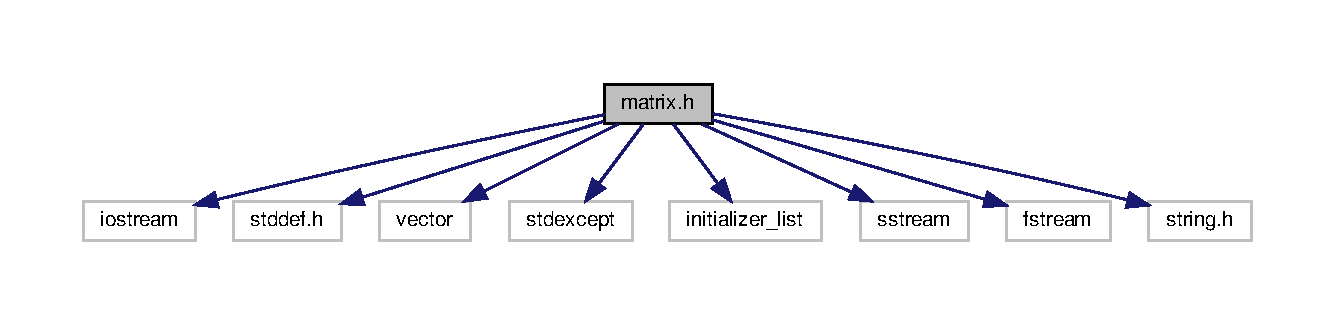
\includegraphics[width=350pt]{matrix_8h__incl}
\end{center}
\end{figure}
\subsection*{Classes}
\begin{DoxyCompactItemize}
\item 
class \hyperlink{classMATOPS_1_1Matrix}{M\+A\+T\+O\+P\+S\+::\+Matrix$<$ T, m, n $>$}
\item 
class \hyperlink{classMATOPS_1_1BigMatrix}{M\+A\+T\+O\+P\+S\+::\+Big\+Matrix$<$ Data1 $>$}
\end{DoxyCompactItemize}
\subsection*{Functions}
\begin{DoxyCompactItemize}
\item 
\mbox{\Hypertarget{matrix_8h_a2050c01cf601a211d3abc45515b8749d}\label{matrix_8h_a2050c01cf601a211d3abc45515b8749d}} 
{\footnotesize template$<$typename Data2 $>$ }\\void {\bfseries M\+A\+T\+O\+P\+S\+::store\+\_\+csv} (Data2 $\ast$$\ast$C, int m\+\_\+1, int n\+\_\+2, std\+::string path)
\item 
\mbox{\Hypertarget{matrix_8h_a058c07f65db98cd52617d3d5c4de3b42}\label{matrix_8h_a058c07f65db98cd52617d3d5c4de3b42}} 
{\footnotesize template$<$typename My\+\_\+data $>$ }\\My\+\_\+data {\bfseries M\+A\+T\+O\+P\+S\+::convert\+\_\+to} (const std\+::string \&str)
\end{DoxyCompactItemize}


\subsection{Detailed Description}
\begin{DoxyDate}{Date}
Jan 9, 2021 
\end{DoxyDate}
\begin{DoxyAuthor}{Author}
Shiladitya Biswas
\end{DoxyAuthor}
\begin{DoxyVerb} This is a simple Matrix operation library, to Multiply and find the transpose of a Matrix.
 The library is divided into two parts, one for small Matrices (i.e. Matrix multiplication
 is performed with O(^3) time complexity) and another for large Matrices where Stressan's
 Algorithm (Time Complexity: O(n^2.8)) is used to Multiply two Matrices.\end{DoxyVerb}

\hypertarget{README_8md}{}\section{R\+E\+A\+D\+M\+E.\+md File Reference}
\label{README_8md}\index{R\+E\+A\+D\+M\+E.\+md@{R\+E\+A\+D\+M\+E.\+md}}

%--- End generated contents ---

% Index
\backmatter
\newpage
\phantomsection
\clearemptydoublepage
\addcontentsline{toc}{chapter}{Index}
\printindex

\end{document}
